\documentclass[a4paper]{article}

\usepackage[dutch]{babel}
\usepackage{a4wide}
\usepackage{enumitem}
\usepackage{graphicx}
\usepackage{tabularx}
\usepackage[titletoc, title]{appendix}
\usepackage{titlesec}
\usepackage{parskip}
\setlength{\parskip}{5pt}

\newcommand{\plus}{\,\texttt{+}\,}
\newcommand{\cpp}{C\texttt{++}}

\newcommand{\specialcell}[2][c]{\begin{tabular}[#1]{@{}l@{}}#2\end{tabular}}
\newcommand{\HRule}{\rule{\linewidth}{0.5mm}}

\setlist[1]{itemsep=0pt}
\usepackage{amsmath}
\usepackage{amssymb}
\usepackage{pdfpages}
\usepackage{tikz}
\usepackage{rotating}
\usepackage{float}
\usepackage{fancyhdr}

\begin{document}

\begin{titlepage}
\center
\textsc{Technische Universiteit Delft}\\[0.2cm]
\textsc{\Huge Bachelor Thesis}\\[1.5cm]
\HRule \\[0.4cm]
{\Huge \bfseries NedTrain Planner}\\[0.5cm]
{\LARGE \bfseries Construeren van Flexibele Roosters}\\[0.4cm]
\HRule \\[1.5cm]

\begin{large}
\begin{minipage}{0.3\textwidth}
\begin{flushleft}
\textit{ \bfseries Auteurs:}\\
\textsc{C. Bakker}\\
\textsc{A. Bouter}\\
\textsc{M. den Hoedt}\\
\end{flushleft}
\end{minipage}
\begin{minipage}{0.6\textwidth}
\begin{flushright}
\textit{ \bfseries Commissie:}\\
\textsc{M.A. Larson} {\normalsize (Vak Co\"ordinator)}\\
\textsc{Prof. Dr. C. Witteveen} {\normalsize (TU Delft Coach)}\\
\textsc{Ir. B. Huisman} {\normalsize (NedTrain)}\\
\end{flushright}
\end{minipage}
\end{large}


\vfill
{\large \today}\\[2cm]

\begin{minipage}{0.48\textwidth}
\begin{flushleft}

\includegraphics[width=0.9\textwidth]{../images/TU_Delft_logo.png}
\end{flushleft}
\end{minipage}
\begin{minipage}{0.48\textwidth}
\begin{flushright}

\includegraphics[width=0.9\textwidth]{../images/NedTrain_logo2.png}
\end{flushright}
\end{minipage}

\end{titlepage}

% \section*{Voorwoord}
Dit verslag is het eindresultaat van het Bachelorproject, dat dient ter afsluiting van de Bachelor Technische Informatica aan de Technische Universiteit Delft. Het project is uitgevoerd in opdracht van het bedrijf NedTrain BV en de TU Delft.

De opdracht bestond uit het implementeren van nieuwe algoritmen, die voort zijn gekomen uit recent onderzoek, en het verbeteren van de NedTrain Planner, een visuele tool voor het oplossen van roosterproblemen. Dit verslag geeft inzicht in de werkzaamheden die door ons uitgevoerd zijn in de tien weken waarin het project plaatsvond. Daarnaast beschrijft het de keuzes die tijdens het proces gemaakt zijn, geeft het de resultaten die behaald zijn en biedt het ondersteuning voor een eventueel vervolgproject.

Wij willen hierbij onze begeleiders ir. Bob Huisman, manager van de Maintenance Development afdeling van NedTrain, en prof. dr. Cees Witteveen, werkzaam bij de Algoritmiek Groep op EWI aan de TU Delft, bedanken voor de feedback op zowel het product als het verslag en het geven van idee\"en en inzichten voor nieuwe functionaliteit. 
\\ \\ \\ \\
\today ~te Delft

Chris Bakker \\
Anton Bouter \\
Martijn den Hoedt


\newpage
\section*{Voorwoord}
Dit verslag is het eindresultaat van het Bachelorproject, dat dient ter afsluiting van de Bachelor Technische Informatica aan de Technische Universiteit Delft. Het project is uitgevoerd in opdracht van het bedrijf NedTrain BV en de TU Delft.

De opdracht bestond uit het implementeren van nieuwe algoritmen, die voort zijn gekomen uit recent onderzoek, en het verbeteren van de NedTrain Planner, een visuele tool voor het oplossen van roosterproblemen. Dit verslag geeft inzicht in de werkzaamheden die door ons uitgevoerd zijn in de tien weken waarin het project plaatsvond. Daarnaast beschrijft het de keuzes die tijdens het proces gemaakt zijn, geeft het de resultaten die behaald zijn en biedt het ondersteuning voor een eventueel vervolgproject.

Wij willen hierbij onze begeleiders ir. Bob Huisman, manager van de Maintenance Development afdeling van NedTrain, en prof. dr. Cees Witteveen, werkzaam bij de Algoritmiek Groep op EWI aan de TU Delft, bedanken voor de feedback op zowel het product als het verslag en het geven van idee\"en en inzichten voor nieuwe functionaliteit. 
\\ \\ \\ \\
\today ~te Delft

Chris Bakker \\
Anton Bouter \\
Martijn den Hoedt


\newpage
\tableofcontents

\newpage
\section*{Samenvatting}

Onze opdrachtgever is NedTrain, onderdeel van de Nederlandse Spoorwegen. Het probleem waarmee NedTrain te maken heeft, staat ook wel bekend als het \emph{Resource Constraint Project Scheduling Problem}. Hierbij wordt er naar een (flexibel) schema gezocht, om bijvoorbeeld treinen te repareren. Doordat elke trein binnen een bepaalde tijd gerepareerd moet worden en er ook rekening gehouden moet worden met de beschikbare resources, is dit probleem zo moeilijk om op te lossen.

De bestaande software van NedTrain bestaat uit een interface, genaamd de NedTrain Planner, en een solver. Hierop hebben wij een aantal aanpassingen gedaan aan de interface. Zo is het nu mogelijk om flexibiliteitsintervallen te zien, staat het sluitknopje op de tab zelf in plaats van in de toolbar en is het mogelijk om activiteiten en resources van plaats te verwisselen. Bovendien is er een aantal bugs verholpen dat de vorige groep heeft achtergelaten. 

De nieuwe solver maakt gebruik van het chaining algoritme en de \emph{COIN Linear Programming} library. Het chaining algoritme is nodig om te zorgen dat bij het verplaatsen van activiteiten het schema consistent is qua resources. De COIN LP library is nodig om flexibiliteitsintervallen te kunnen berekenen, die vervolgens worden weergegeven in de interface. 

Tijdens dit project hebben we gebruik gemaakt van scrum en zes wekelijkse sprints. Als versiebeheersysteem gebruikten wij Git op een private repository gehost door \href{http://bitbucket.com}{Bitbucket.com}, wat erg prettig heeft gewerkt. Als continuous integration systeem hebben een server met daarop Jenkins, maar dit was helaas geen succes. De codekwaliteit is gemeten door de Software Improvement Group, die vervolgens feedback heeft gegeven over verschillende aspecten van de code. 

We hebben een viertal aanbevelingen voor personen die de NedTrain Planner gaan doorontwikkelen. We bevelen aan om een undo-functionaliteit te maken, de communicatie tussen interface en solver sneller te maken, de code kwaliteit te verbeteren en visueel te maken welke resource unit wanneer nodig is. 

TODO: conclusie

\newpage
\pagestyle{fancy}
\fancyhead[L]{}
\section{Inleiding}
Dit verslag is het eindresultaat van het Bachelorproject in opdracht van NedTrain B.V. en de Technische Universiteit Delft. Het project was gericht op het uitbreiden en verbeteren van software voor een applicatie, de NedTrain Planner, die roosterproblemen kan oplossen en de uitkomsten hiervan op een overzichtelijk manier visualiseren. De applicatie kan voor verschillende doeleinden gebruikt worden door zowel NedTrain als de TU Delft. Er moet dus tijdens het project rekening worden gehouden met verschillende belangen en wensen van beide opdrachtgevers.

In de komende hoofdstukken zal de opdracht en het proces eromheen beschreven worden. Allereerst zal er gedefini\"eerd worden wat het probleem van de opdrachtgevers is. Vervolgens zal het hoofdstuk probleemanalyse gericht zijn op het analyseren en oplossen van het gedefini\"eerde probleem van de opdrachtgevers. Daarna zullen in het hoofdstuk ontwerp de ontwerpkeuzes genoemd en toegelicht worden en komen in het daarop volgende hoofdstuk alle opgeleverde producten en diensten aan bod. Omdat de applicatie gericht is op het oplossen van problemen zal er ook een hoofdstuk gewijd zijn aan de performance van de opgeleverde producten. Vervolgens zal besproken worden hoe het ontwikkelproces gelopen is en wat voor hulpmiddelen er gebruikt zijn. Tenslotte zullen er functionaliteiten aanbevolen worden die eventueel later nog ge\"implementeerd kunnen worden en wordt in de conclusie teruggekeken op het project en een conclusie getrokken met betrekking tot de eisen van het project. Als voorbereiding op dit project zijn in de eerste weken een aantal documenten opgesteld, namelijk een Plan van Aanpak \emph{(zie bijlage \ref{app:B})}, een Ori\"entatieverslag \emph{(zie bijlage \ref{app:C})} en een Requirementsanalyse \emph{(zie Bijlage \ref{app:D})}

De volgende paragrafen zullen een korte inleiding geven over het bedrijf NedTrain en waarom de NedTrain Planner relevant is voor hen en de TU Delft.

\subsection{NedTrain}
Het bedrijf NedTrain is een dochterbedrijf van de Nederlandse Spoorwegen (NS), net als bijvoorbeeld NS Reizigers B.V., de verantwoordelijke voor het personenvervoer. NedTrain is het dochterbedrijf dat zorgt voor het onderhoud aan alle treinen aangeleverd door NS Reizigers. Dat onderhoud bestaat niet alleen uit het repareren, maar ook uit het reinigen en moderniseren van treinen. Er moet hierbij gezorgd worden dat van de grofweg 3000 bestaande treinstellen bij NS er op elk moment genoeg beschikbaar zijn om gebruikt te kunnen worden door NS Reizigers. Om dit te bereiken staan er op elk moment van de dag ongeveer 250 treinstellen tegelijk voor onderhoud op meer dan 30 locaties door heel Nederland in de werkplaatsen van NedTrain. Hier werken in totaal ongeveer 3500 mensen 24 uur per dag, 7 dagen per week aan de opgenoemde taken. Het hoofdkantoor van NedTrain staat in Utrecht.

\subsection{NedTrain Planner}
Vanwege de omvang van de activiteiten, die NedTrain dagelijks moet afhandelen, worden er roosters gemaakt die een weergave van de dag geven en er voor moeten zorgen dat deze activiteiten op tijd uitgevoerd worden. Dit is een uitputtende taak en alhoewel NedTrain in het bezit is van software moet er nog steeds veel met de hand worden gedaan. Om NedTrain te helpen bij het inzicht geven van de nieuwste ontwikkelingen rondom het oplossen van moeilijke roosterproblemen is er in samenwerking met de TU Delft de NedTrain Planner ontwikkeld, dat het resultaat is van meerdere projecten van studenten aan de TU Delft. Roostermakers bij NedTrain zouden deze applicatie kunnen gebruiken om hun werkverrichtingen te vergemakkelijken en hun denkwijze te verbeteren. Daarnaast biedt het voor de TU Delft een educatief demonstratiemiddel voor onderzoek, doordat de applicatie visueel goed kan laten zien hoe de oplossing door een algoritme tot stand komt en hoe dus een dergelijk algoritme werkt.

\newpage
\section{Probleemstelling}
\label{sec:probleemstelling}

De NedTrain Planner is een uitgebreide grafische applicatie waarin roosterproblemen kunnen worden aangemaakt, ge\"importeerd, gevisualiseerd en aangepast. Door middel van een zogenaamde solver, die onafhankelijk is van de gebruikersinterface en die ingeladen moet worden in de applicatie, kunnen deze roosterproblemen opgelost worden. Vervolgens kan er informatie verkregen en opgevraagd worden over de gevonden oplossing en kan er stapsgewijs door het proces van de solver heen gelopen worden om zo een betere overzicht te krijgen over hoe de solver werkt. Daarnaast geeft de NedTrain Planner API ook de mogelijk om na het oplossen aanpassingen te maken en dit opnieuw op te laten lossen door de solver om zo veranderingen in gedrag en resultaat te weergeven.

E\'en van de mogelijkheden die de NedTrain Planner biedt na het oplossen is het verschuiven van activiteiten over hun uitvoerbare intervallen. Deze intervallen tonen aan in hoeverre activiteiten verschoven kunnen worden, zonder dat dit leidt tot een onhaalbare oplossing. Echter biedt de huidige solver alleen garantie dat als alle activiteiten op hun vroegste starttijd staan, dat dit een haalbare oplossing is voor het gegeven probleem. Het is dus mogelijk dat er bij het verschuiven van een activiteit een capaciteit van een resource overschreden wordt.

Het eerste gedeelte van het probleem is om een algoritme te implementeren die garandeert dat voor elke tijdsbepaling van de activiteiten dit niet een onhaalbaar rooster geeft. Er moet dus uiteindelijk met de activiteiten over hun uitvoerbare intervallen verschoven kunnen worden, zonder dat er een resource zijn capaciteit overschreidt of dat er een beperking geschonden wordt.

Het tweede gedeelte van het probleem is om de NedTrain Planner uit te breiden met functionaliteit die er voor zorgt dat er flexibele roosters geconstrueerd en gevisualiseerd kunnen worden. Dit betekend dat activiteiten vrij over een interval moeten kunnen bewegen zonder dat daarbij de starttijd of vorm van een andere activiteit veranderd wordt. Dit geeft NedTrain de mogelijkheid om bij het uitvoeren van een rooster makkelijk aanpassingen te kunnen maken, zonder daarbij het hele rooster hoeven te veranderen of opnieuw te berekenen.

Het laatste gedeelte van het probleem is om informatie te geven over de flexibiliteit en het berekenen hiervan. Daarnaast moeten veranderingen in deze informatie ge\"evalueerd kunnen worden na het geven van gebruikersfeedback. Dit kan door de TU Delft gebruikt worden om beter te begrijpen hoe de algoritmes zich gedragen en kan het helpen om verdere onderzoek naar het oplossen van roosterproblemen te stimuleren.




\newpage
\section{Probleemanalyse}
\label{sec:probleemanalyse}

Het probleem dat in Hoofdstuk \ref{sec:probleemstelling} ge\"introduceerd is, zal in dit hoofdstuk formeel gedefini\"eerd worden. Vervolgens zullen voor de verschillende onderdelen van het probleem oplosmethoden besproken worden.

\subsection{Resource Constraint Project Scheduling Problem}
Het probleem waar NedTrain mee te maken heeft, staat ook wel bekend als het \emph{Resource Constraint Project Scheduling Problem (RCPSP)}. Zo'n probleem gaat om het inplannen van activiteiten die elk bepaalde resources nodig hebben, zonder dat de maximale capaciteit van de resources geschonden wordt. De instanties van NedTrain bestaan uit projecten $P = \{p_1, \dots , p_n\}$ die uit \'e\'en of meer subactiviteiten $v_{a,b}$ bestaan. De verzameling van alle activiteiten, $\bigcup_{\{p_a \in P\}} V_a$, wordt gedefinieerd als de verzameling $V = \{v_{1,1}, \dots , v_{n,m}\}$. Een project $p_a$ heeft een starttijd \emph{(release time)} $rs_a$ en een deadline $dl_a$. De subactiviteiten van project $p_a$ mogen pas vanaf $rs_a$ uitgevoerd worden, maar moeten wel uiterlijk op $dl_a$ klaar zijn. De b$^e$ activiteit van project $p_a$ wordt weergegeven als $v_{a,b}$. Deze activiteit heeft een tijdsduur van $d_{a,b}$ tijdseenheden.

Er zijn drie soorten voorwaarden \emph{(constraints)} waar rekening mee gehouden moet worden bij het oplossen van RCPSP. Dit zijn tijdsconstraints, voorrangsrelaties (precedence constraints) en resource constraints. De tijdsconstraints zijn de hierboven genoemde starttijden en deadlines van de projecten. Een eventuele voorrangsrelatie $v_{i,j} \prec v_{u,v}$ kan bestaan tussen twee activiteiten $v_{i,j}$ en $v_{u,v}$, waardoor activiteit $v_{i,j}$ voltooid moet zijn, voordat activiteit $v_{u,v}$ uitgevoerd mag worden. Tenslotte zijn oplossingen ook gelimiteerd door de resource constraints. Elke taak kan namelijk van verschillende soorten resources $r_k$ een bepaald aantal units nodig hebben. Het aantal units dat activiteit $v_{i,j}$ van resource $r_k$ nodig heeft, wordt genoteerd als $req(v_{i,j},r_k)$.

Een formele definitie van RCPSP kan nu als volgt opgesteld worden:

\textbf{Gegeven:}\\
Een verzameling projecten $P = \{p_1, \dots ,p_n\}$ met voor elk project $p_a$ een starttijd $rs_a$, een deadline $dl_a$ en een verzameling activiteiten $V_a = \{v_{a,1},\dots ,v_{a,m}\}$ met voor elke activiteit $v_{a,b}$ een tijdsduur $d_{a,b}$. Daarnaast een verzameling van voorrangsrelaties $E \subseteq V \times V = \{(v_{a,b},v_{c,d}) | v_{a,b} \in V_a \wedge v_{c,d} \in V_c \wedge p_a,p_c \in P \}$, een verzameling van $w$ resources $R = \{r_1, \dots ,r_w\}$ met voor elke resource $r_i$ een eindige capaciteit $cap(r_i)$, en voor elke activiteit $v_{a,b} \in \bigcup_{\{p_a \in P\}} V_a$ een hoeveelheid van resource $r_k \in R$ die nodig is, $req(v_{a,b},r_k)$.

\textbf{Vind:}\\
Een doenlijk schema $S = \{s_1,\dots ,s_m\}$ bestaande uit starttijden $s_{a,b}$ voor elke activiteit $v_{a,b} \in V$, zodat $rs_a \leq s_{a,b} \wedge s_{a,b} + d_{a,b} \leq dl_a$, waarbij voor elke voorrangsrelatie $(v_{a,b},v_{c,d}) \in E$ geldt dat $s_{a,b} + d_{a,b} \leq s_{c,d}$. Bovendien mag op geen enkel tijdstip de capaciteit van een resource overschreden worden, wat inhoudt dat $\forall r_i \in R$ en $\forall t \in \mathbb{R}$ geldt dat $\Sigma _{\{v_{a,b} \in V | s_{a,b} \leq t \leq s_{a,b} + d_{a,b}\}} req(v_{a,b},r_i) \leq cap(r_i)$.

\subsection{Flexibiliteit}
Omdat de huidige software al een oplossing voor het RCPSP kan vinden, is aan ons de taak om deze oplossing flexibeler te maken. Daarvoor moet dus eerst de flexibiliteit van een schema gedefini\"eerd worden. Hiervoor zal de flexibiliteitsmaat van Wilson \emph{et al.} \cite{wilson2013flexibility} gebruikt worden, omdat deze maat er ook rekening mee houdt dat een schema minder flexibel wordt door het toevoegen van voorrangsrelaties. Om deze te berekenen, moet voor elke activiteit $v_{a,b}$ een interval $[l_v,u_v]$ berekend worden, zodat elke activiteit in zijn eigen interval verschoven kan worden, zonder dat daardoor andere activiteiten verplaatst hoeven te worden. Dit houdt dus in dat de verzameling van intervallen $I_S = \{I_v = [l_v,u_v] | v \in V\}$ voldoet desda voor elke $v \in V$ en voor elke $t_v \in [l_v,u,v]$, een toewijzing van starttijd $t_v$ aan activiteit $v$ een consistent schema oplevert. Vervolgens kan de flexibiliteit van het schema berekend worden door de lengtes van de intervallen bij elkaar op te tellen, zoals in formule \ref{eq:flex1}:

\begin{align}
\label{eq:flex1}
    flex = \sum_{v \in V} (u_v - l_v)
\end{align}

\subsection{Oplossing}
\label{subsec:probleemoplossing}
In de bestaande software was al een algoritme ge\"implementeerd dat een doenlijk schema kan vinden door middel van het ESTA$^+$ algoritme \cite{ronaldevers2010}.
Dit algoritme lost het RCPSP op door het vinden en oplossen van \emph{contention peaks}, plekken in het resource profiel waar er meer resource units gebruikt worden dan er beschikbaar zijn. Deze worden veroorzaakt doordat er te veel activiteiten die dezelfde resource gebruiken tegelijk uitgevoerd worden en kunnen opgelost worden door tussen minstens 1 paar van deze activiteiten een voorrangsrelatie toe te voegen. Het $ESTA^+$ algoritme levert als oplossing voor elke activiteit een starttijd, zodat het gehele schema consistent is. Als er met activiteiten geschoven wordt, kan het schema echter nog wel inconsistent worden.

\subsubsection{Chaining}
\label{subsubsec:chainingoplossing}
Om onafhankelijke flexibiliteitsintervallen te kunnen bepalen, moeten activiteiten echter vrij verschoven kunnen worden, zonder dat hierdoor het schema inconsistent wordt. Hier kan het chaining algoritme voor zorgen. Dit algoritme wijst aan elke resource unit een zogenaamde chain, een gesorteerde lijst van activiteiten, toe. In een chain geldt voor elk paar opeenvolgende activiteiten, $v_{a,b}$ en $v_{c,d}$, dat er een voorrangsrelatie $v_{a,b} \prec v_{c,d}$ bestaat. De output van het chaining algoritme bestaat uit een \emph{Partial Order Schedule (POS)}, wat een schema is waarvoor geldt dat elk schema dat qua tijdsconstraints consistent is, ook consistent is met de resource constraints. Het exact chaining algoritme is weergegeven in Algoritme \ref{alg:chaining}.

\begin{algorithm}
\caption{Chaining \cite{policella2007precedence}}
\label{alg:chaining}
\textbf{Input:} A problem P and one of its fixed-times schedules $S$ \\
\textbf{Output:} A partial order solution $POS^{ch}$
\begin{algorithmic}[1]
  \Function{Chaining}{$P, S$}
    \Let{$POS^{ch}$}{$P$}
    \State Sort all the activities according to their start times in $S$  
    \State Initialize all the chains empty
    \For{\textbf{each} resource $r_j$}
      \For{\textbf{each} activity $v_i$}
        \For{$1$ \textbf{to} $req_{ij}$}
          \Let{$k$}{$SelectChain(v_i,r_j)$}
          \Let{$v_k$}{$last(k)$}
          \State{$AddConstraint(POS^{ch},v_k \prec v_i)$}
          \Let{$last(k)$}{$v_i$}
        \EndFor
      \EndFor
    \EndFor
    \State{\Return{$POS^{ch}$}}
  \EndFunction
\end{algorithmic}
\end{algorithm}

In de functie $SelectChain(v_i,r_j)$ wordt een chain gekozen waar activiteit $v_i$ aan toegevoegd zal worden. Een simpele, voor de hand liggende methode is om een activiteit gelijk aan een chain toe te voegen als er een geschikte chain gevonden is. Een chain is geschikt voor een activiteit $v_i$ als de eindtijd van het laatste element van de chain, $v_k$, eerder is dan de starttijd van $v_i$, dus $s_k + d_k \leq s_i$. Er kan ook voor gekozen worden om een willekeurige chain te selecteren. Hiervoor moeten eerst alle geschikte chains gevonden worden, en wordt er vervolgens uit deze verzameling een willekeurig element gekozen. Tenslotte is er ook in \cite{policella2004generating} een heuristiek voorgesteld die probeert om het aantal voorrangsrelaties tussen activiteiten uit verschillende chains te minimaliseren. Deze heuristiek, weergegeven in \ref{alg:selectchain1}, selecteert voor een activiteit eerst een willekeurige chain $k$  en voegt dan een voorrangsrelatie toe tussen $v_i$ en het laatste element van $k$, $last(k)$. Als $v_i$ nog meer units van dezelfde resource nodig heeft, wordt er eerst geprobeerd om $v_i$ aan chains toe te voegen die ook $last(k)$ als laatste element hebben, omdat er dan geen nieuwe voorrangsrelatie toegevoegd hoeft te worden. De voorrangsrelatie $v_i \prec last(k)$ bestaat immers al. Hierna komen pas andere chains, die $last(k)$ niet als laatste element hebben, in aanmerking voor activiteit $v_i$.

\begin{algorithm}
\caption{SelectChain Heuristiek \cite{policella2004generating}}
\label{alg:selectchain1}
\textbf{Input:} Een probleeminstantie $P$, een activiteit $v_i$ en een resource $r_j$. \\
\begin{algorithmic}[1]
  \Function{SelectChain}{$P, v_i, r_j$}
    \State Selecteer een willekeurige geschikte chain $k$
    \State{$AddConstraint(P,v_k \prec v_i)$}
    \If{$req(v_i,r_j) > 0$}
    		\Let{$C_k, \overline{C_k}$}{$\emptyset$}
    		\For{\textbf{each} chain $c$}
    			\If{$last(c) == last(k)$}
    				\Let{$C_k$}{$C_k \cup c$}
    			\Else
    				\Let{$\overline{C_k}$}{$\overline{C_k} \cup c$}
    			\EndIf
    		\EndFor
    		\For{$req = req(v_i,r_j)-1 \dots 0$}
    			\If{$C_k \neq \emptyset$}
    				\Let{$v_k$}{willekeurig element in $C_k$}
    				\State{$AddConstraint(P,v_k \prec v_i)$}
    				\Let{$C_k$}{$C_k - v_k$}
    			\Else
    				\Let{$v_k$}{willekeurig element in $\overline{C_k}$}
    				\State{$AddConstraint(P,v_k \prec v_i)$}
    				\Let{$\overline{C_k}$}{$\overline{C_k} - v_k$}
    			\EndIf
    		\EndFor
    	\EndIf
  \EndFunction
\end{algorithmic}
\end{algorithm}

\subsubsection{Linear Programming}
\label{subsubsec:flexoplossing}
Nu alle constraints door het chaining algoritme aan het model zijn toegevoegd, kan de flexibiliteit van het schema worden geoptimaliseerd, door de probleeminstantie om te zetten naar een Linear Programming probleem (LP-probleem). Dit probleem kan in polynomiale tijd opgelost worden door middel van een LP-solver.

De flexibiliteit van een taak $flex = t^+ - t^-$, waarbij $t^+$ de laatste starttijd (l.s.t.) en $t^-$ de eerste starttijd (e.s.t.) van een taak $t$ is. De flexibiliteit van het hele schema wordt gemeten door de som van de flexibiliteit van alle taken $t \in T$ te nemen, zoals in formule \ref{eq:flex} is weergegeven. 

\begin{align}
\label{eq:flex}
    flex_{totaal} = \sum_{t \in T} (t^+ - t^-)
\end{align}

Het doel is de flexibiliteit te maximaliseren en ervoor te zorgen dat er tegelijkertijd wordt voldaan aan de constraints $(t - t' \leq c) \in C$. Ook mag de e.s.t. niet na de l.s.t. zijn ($t^- \leq t^+ \Rightarrow 0 \leq t^+ - t^-$). Hieruit volgt het LP-probleem zoals in formule \ref{eq:flexLP} staat.

\begin{align}
\label{eq:flexLP}
\begin{aligned}
        \text{max:}& \quad \sum_{t \in T} (t^+ - t^-) & \\
 \text{subject to:}& \quad 0 \leq t^+ - t^- & \forall t \in T \\
                   & \quad t^+ - t^- \leq c & \forall (t^+ - t^{'-} \leq c) \in C
\end{aligned}
\end{align}

Het nadeel van de formulering in formule \ref{eq:flexLP}, is dat de flexibiliteit  niet netjes verdeeld hoeft te zijn over de taken. Wij hebben gezien dat CLP meestal de flexibiliteit juist heel slecht verdeelt. Met het LP-probleem, zoals in formule \ref{eq:flexfirstLP} staat, wordt de minimale flexibiliteit $min$ gemaximaliseerd. Vervolgens wordt met LP-probleem, zoals in formule \ref{eq:flexsecondLP} staat, de totale flexibiliteit gemaximaliseerd. Dit is eigenlijk hetzelfde als in formule \ref{eq:flexLP}, maar nu met als nieuwe voorwaarde dat elke taak minimaal een flexibiliteit van $min$ moet hebben ($min \leq t^+ - t^ -$). 

\begin{align}
\label{eq:flexfirstLP}
\begin{aligned}
        \text{max:}& \quad min & \\
 \text{subject to:}& \quad min \leq t^+ - t^- & \forall t \in T \\
                   & \quad t^+ - t'^- \leq c & \forall (t - t' \leq c) \in C
\end{aligned}
\end{align}

\begin{align}
\label{eq:flexsecondLP}
\begin{aligned}
        \text{max:}& \quad \sum_{t \in T} (t^+ - t^-) & \\
 \text{subject to:}& \quad min \leq t^+ - t^- & \forall t \in T \\
                   & \quad t^+ - t'^- \leq c & \forall (t - t' \leq c) \in C
\end{aligned}
\end{align}

Door het toevoegen van de nieuwe constraint $min \leq t^+ - t^-$, kan het zijn dat de totale flexibiliteit $flex_{totaal}$ minder is dan bij het gebruik van formule \ref{eq:flexLP}, maar nu is de flexibiliteit wel beter verdeeld.
\newpage
\section{Ontwerp}
\subsection{Solver}
Als de gebruiker op de knop 'solve' drukt, wordt de solver aangeroepen. Deze leest de probleeminstantie in en verwerkt deze. Uiteindelijk geeft de solver weer informatie terug aan de tool, die de informatie weergeeft op het scherm. Deze informatie bestaat onder andere uit de chains en de flexibiliteitsintervallen.

De solver bestaat grofweg uit drie componenten, namelijk het ESTA$^+$ algoritme, het chaining algoritme en een algoritme voor het berekenen van de flexibiliteitsintervallen. Het ESTA$^+$ algoritme was al ge\"implementeerd door onze voorgangers en hieraan hebben wij ook niets veranderd. Het chaining algoritme, uitgelegd in paragraaf \ref{subsubsec:chainingoplossing}, hebben we zelf ge\"implementeerd. De code voor het berekenen van de flexibiliteitsintervallen bouwt een LP-probleem op en lost deze vervolgens op met de COIN LP (Clp) library. Hoe de solver werkt en wat voor aanroepen er gedaan worden, is weergegeven in het sequencediagram in Figuur \ref{fig:sd}.

\newpage
\begin{figure}[H]
\centering
\label{fig:sd}
\ifx\du\undefined
  \newlength{\du}
\fi
\setlength{\du}{15\unitlength}
\begin{sideways}
\begin{tikzpicture}
\pgftransformxscale{1.000000}
\pgftransformyscale{-1.000000}
\definecolor{dialinecolor}{rgb}{0.000000, 0.000000, 0.000000}
\pgfsetstrokecolor{dialinecolor}
\definecolor{dialinecolor}{rgb}{1.000000, 1.000000, 1.000000}
\pgfsetfillcolor{dialinecolor}
\pgfsetlinewidth{0.100000\du}
\pgfsetdash{}{0pt}
\definecolor{dialinecolor}{rgb}{1.000000, 1.000000, 1.000000}
\pgfsetfillcolor{dialinecolor}
\fill (29.069200\du,8.000000\du)--(29.069200\du,30.000000\du)--(46.069200\du,30.000000\du)--(46.069200\du,8.000000\du)--cycle;
\definecolor{dialinecolor}{rgb}{0.000000, 0.000000, 0.000000}
\pgfsetstrokecolor{dialinecolor}
\draw (29.069200\du,8.000000\du)--(29.069200\du,30.000000\du)--(46.069200\du,30.000000\du)--(46.069200\du,8.000000\du)--cycle;
\definecolor{dialinecolor}{rgb}{1.000000, 1.000000, 1.000000}
\pgfsetfillcolor{dialinecolor}
\fill (29.069200\du,7.000000\du)--(29.069200\du,8.000000\du)--(31.579200\du,8.000000\du)--(31.579200\du,7.000000\du)--cycle;
\definecolor{dialinecolor}{rgb}{0.000000, 0.000000, 0.000000}
\pgfsetstrokecolor{dialinecolor}
\draw (29.069200\du,7.000000\du)--(29.069200\du,8.000000\du)--(31.579200\du,8.000000\du)--(31.579200\du,7.000000\du)--cycle;
% setfont left to latex
\definecolor{dialinecolor}{rgb}{0.000000, 0.000000, 0.000000}
\pgfsetstrokecolor{dialinecolor}
\node[anchor=west] at (29.169200\du,7.600000\du){Solver};
\pgfsetlinewidth{0.000000\du}
\pgfsetdash{}{0pt}
\pgfsetdash{}{0pt}
\pgfsetmiterjoin
\definecolor{dialinecolor}{rgb}{1.000000, 1.000000, 1.000000}
\pgfsetfillcolor{dialinecolor}
\fill (45.984921\du,21.864133\du)--(45.984921\du,22.599904\du)--(46.126761\du,22.599904\du)--(46.126761\du,21.864133\du)--cycle;
\definecolor{dialinecolor}{rgb}{1.000000, 1.000000, 1.000000}
\pgfsetstrokecolor{dialinecolor}
\draw (45.984921\du,21.864133\du)--(45.984921\du,22.599904\du)--(46.126761\du,22.599904\du)--(46.126761\du,21.864133\du)--cycle;
\pgfsetlinewidth{0.000000\du}
\pgfsetdash{}{0pt}
\pgfsetdash{}{0pt}
\pgfsetmiterjoin
\definecolor{dialinecolor}{rgb}{1.000000, 1.000000, 1.000000}
\pgfsetfillcolor{dialinecolor}
\fill (46.000640\du,19.882377\du)--(46.000640\du,20.567260\du)--(46.142480\du,20.567260\du)--(46.142480\du,19.882377\du)--cycle;
\definecolor{dialinecolor}{rgb}{1.000000, 1.000000, 1.000000}
\pgfsetstrokecolor{dialinecolor}
\draw (46.000640\du,19.882377\du)--(46.000640\du,20.567260\du)--(46.142480\du,20.567260\du)--(46.142480\du,19.882377\du)--cycle;
\pgfsetlinewidth{0.000000\du}
\pgfsetdash{}{0pt}
\pgfsetdash{}{0pt}
\pgfsetmiterjoin
\definecolor{dialinecolor}{rgb}{1.000000, 1.000000, 1.000000}
\pgfsetfillcolor{dialinecolor}
\fill (28.994166\du,12.926291\du)--(28.994166\du,13.611175\du)--(29.136006\du,13.611175\du)--(29.136006\du,12.926291\du)--cycle;
\definecolor{dialinecolor}{rgb}{1.000000, 1.000000, 1.000000}
\pgfsetstrokecolor{dialinecolor}
\draw (28.994166\du,12.926291\du)--(28.994166\du,13.611175\du)--(29.136006\du,13.611175\du)--(29.136006\du,12.926291\du)--cycle;
\pgfsetlinewidth{0.050000\du}
\pgfsetdash{}{0pt}
\pgfsetdash{{0.400000\du}{0.400000\du}}{0\du}
\definecolor{dialinecolor}{rgb}{0.000000, 0.000000, 0.000000}
\pgfsetstrokecolor{dialinecolor}
\draw (23.683300\du,10.875000\du)--(23.683300\du,12.275000\du);
\definecolor{dialinecolor}{rgb}{0.000000, 0.000000, 0.000000}
\pgfsetstrokecolor{dialinecolor}
\draw (23.683300\du,26.275000\du)--(23.683300\du,29.983241\du);
\pgfsetlinewidth{0.100000\du}
\pgfsetdash{}{0pt}
\definecolor{dialinecolor}{rgb}{1.000000, 1.000000, 1.000000}
\pgfsetfillcolor{dialinecolor}
\fill (23.333300\du,12.275000\du)--(23.333300\du,26.275000\du)--(24.033300\du,26.275000\du)--(24.033300\du,12.275000\du)--cycle;
\definecolor{dialinecolor}{rgb}{0.000000, 0.000000, 0.000000}
\pgfsetstrokecolor{dialinecolor}
\draw (23.333300\du,12.275000\du)--(23.333300\du,26.275000\du)--(24.033300\du,26.275000\du)--(24.033300\du,12.275000\du)--cycle;
\pgfsetlinewidth{0.100000\du}
\pgfsetdash{}{0pt}
\definecolor{dialinecolor}{rgb}{1.000000, 1.000000, 1.000000}
\pgfsetfillcolor{dialinecolor}
\pgfpathellipse{\pgfpoint{16.050000\du}{6.250000\du}}{\pgfpoint{0.300000\du}{0\du}}{\pgfpoint{0\du}{0.300000\du}}
\pgfusepath{fill}
\definecolor{dialinecolor}{rgb}{0.000000, 0.000000, 0.000000}
\pgfsetstrokecolor{dialinecolor}
\pgfpathellipse{\pgfpoint{16.050000\du}{6.250000\du}}{\pgfpoint{0.300000\du}{0\du}}{\pgfpoint{0\du}{0.300000\du}}
\pgfusepath{stroke}
\definecolor{dialinecolor}{rgb}{0.000000, 0.000000, 0.000000}
\pgfsetstrokecolor{dialinecolor}
\draw (14.850000\du,6.850000\du)--(17.250000\du,6.850000\du);
\definecolor{dialinecolor}{rgb}{0.000000, 0.000000, 0.000000}
\pgfsetstrokecolor{dialinecolor}
\draw (16.050000\du,6.550000\du)--(16.050000\du,8.050000\du);
\definecolor{dialinecolor}{rgb}{0.000000, 0.000000, 0.000000}
\pgfsetstrokecolor{dialinecolor}
\draw (16.050000\du,8.050000\du)--(14.850000\du,9.350000\du);
\definecolor{dialinecolor}{rgb}{0.000000, 0.000000, 0.000000}
\pgfsetstrokecolor{dialinecolor}
\draw (16.050000\du,8.050000\du)--(17.250000\du,9.350000\du);
% setfont left to latex
\definecolor{dialinecolor}{rgb}{0.000000, 0.000000, 0.000000}
\pgfsetstrokecolor{dialinecolor}
\node at (16.050000\du,10.445000\du){Gebruiker};
\pgfsetlinewidth{0.100000\du}
\pgfsetdash{}{0pt}
\definecolor{dialinecolor}{rgb}{1.000000, 1.000000, 1.000000}
\pgfsetfillcolor{dialinecolor}
\fill (21.500000\du,8.609620\du)--(25.265000\du,8.609620\du)--(25.865000\du,9.209620\du)--(25.865000\du,10.309620\du)--(21.500000\du,10.309620\du)--cycle;
\definecolor{dialinecolor}{rgb}{0.000000, 0.000000, 0.000000}
\pgfsetstrokecolor{dialinecolor}
\draw (21.500000\du,8.609620\du)--(25.265000\du,8.609620\du)--(25.865000\du,9.209620\du)--(25.865000\du,10.309620\du)--(21.500000\du,10.309620\du)--cycle;
\pgfsetlinewidth{0.050000\du}
\definecolor{dialinecolor}{rgb}{0.000000, 0.000000, 0.000000}
\pgfsetstrokecolor{dialinecolor}
\draw (25.265000\du,8.609620\du)--(25.265000\du,9.209620\du)--(25.865000\du,9.209620\du);
% setfont left to latex
\definecolor{dialinecolor}{rgb}{0.000000, 0.000000, 0.000000}
\pgfsetstrokecolor{dialinecolor}
\node[anchor=west] at (21.850000\du,9.754620\du){Interface};
\pgfsetlinewidth{0.100000\du}
\pgfsetdash{}{0pt}
\definecolor{dialinecolor}{rgb}{1.000000, 1.000000, 1.000000}
\pgfsetfillcolor{dialinecolor}
\fill (29.700000\du,8.609620\du)--(31.925000\du,8.609620\du)--(32.525000\du,9.209620\du)--(32.525000\du,10.309620\du)--(29.700000\du,10.309620\du)--cycle;
\definecolor{dialinecolor}{rgb}{0.000000, 0.000000, 0.000000}
\pgfsetstrokecolor{dialinecolor}
\draw (29.700000\du,8.609620\du)--(31.925000\du,8.609620\du)--(32.525000\du,9.209620\du)--(32.525000\du,10.309620\du)--(29.700000\du,10.309620\du)--cycle;
\pgfsetlinewidth{0.050000\du}
\definecolor{dialinecolor}{rgb}{0.000000, 0.000000, 0.000000}
\pgfsetstrokecolor{dialinecolor}
\draw (31.925000\du,8.609620\du)--(31.925000\du,9.209620\du)--(32.525000\du,9.209620\du);
% setfont left to latex
\definecolor{dialinecolor}{rgb}{0.000000, 0.000000, 0.000000}
\pgfsetstrokecolor{dialinecolor}
\node[anchor=west] at (30.050000\du,9.754620\du){ESTA+};
\pgfsetlinewidth{0.050000\du}
\pgfsetdash{}{0pt}
\pgfsetdash{{0.400000\du}{0.400000\du}}{0\du}
\definecolor{dialinecolor}{rgb}{0.000000, 0.000000, 0.000000}
\pgfsetstrokecolor{dialinecolor}
\draw (16.070000\du,10.875000\du)--(16.070000\du,12.275000\du);
\definecolor{dialinecolor}{rgb}{0.000000, 0.000000, 0.000000}
\pgfsetstrokecolor{dialinecolor}
\draw (16.070000\du,28.275000\du)--(16.070000\du,30.000000\du);
\pgfsetlinewidth{0.100000\du}
\pgfsetdash{}{0pt}
\definecolor{dialinecolor}{rgb}{1.000000, 1.000000, 1.000000}
\pgfsetfillcolor{dialinecolor}
\fill (15.720000\du,12.275000\du)--(15.720000\du,28.275000\du)--(16.420000\du,28.275000\du)--(16.420000\du,12.275000\du)--cycle;
\definecolor{dialinecolor}{rgb}{0.000000, 0.000000, 0.000000}
\pgfsetstrokecolor{dialinecolor}
\draw (15.720000\du,12.275000\du)--(15.720000\du,28.275000\du)--(16.420000\du,28.275000\du)--(16.420000\du,12.275000\du)--cycle;
\pgfsetlinewidth{0.050000\du}
\pgfsetdash{}{0pt}
\pgfsetdash{{0.400000\du}{0.400000\du}}{0\du}
\definecolor{dialinecolor}{rgb}{0.000000, 0.000000, 0.000000}
\pgfsetstrokecolor{dialinecolor}
\draw (31.100000\du,10.171800\du)--(31.100000\du,12.776672\du);
\definecolor{dialinecolor}{rgb}{0.000000, 0.000000, 0.000000}
\pgfsetstrokecolor{dialinecolor}
\draw (31.100000\du,16.776672\du)--(31.100000\du,30.000000\du);
\pgfsetlinewidth{0.100000\du}
\pgfsetdash{}{0pt}
\definecolor{dialinecolor}{rgb}{1.000000, 1.000000, 1.000000}
\pgfsetfillcolor{dialinecolor}
\fill (30.750000\du,12.776672\du)--(30.750000\du,16.776672\du)--(31.450000\du,16.776672\du)--(31.450000\du,12.776672\du)--cycle;
\definecolor{dialinecolor}{rgb}{0.000000, 0.000000, 0.000000}
\pgfsetstrokecolor{dialinecolor}
\draw (30.750000\du,12.776672\du)--(30.750000\du,16.776672\du)--(31.450000\du,16.776672\du)--(31.450000\du,12.776672\du)--cycle;
\pgfsetlinewidth{0.050000\du}
\pgfsetdash{}{0pt}
\pgfsetdash{{0.400000\du}{0.400000\du}}{0\du}
\definecolor{dialinecolor}{rgb}{0.000000, 0.000000, 0.000000}
\pgfsetstrokecolor{dialinecolor}
\draw (49.797500\du,10.100300\du)--(49.797500\du,19.790678\du);
\definecolor{dialinecolor}{rgb}{0.000000, 0.000000, 0.000000}
\pgfsetstrokecolor{dialinecolor}
\draw (49.797500\du,21.790678\du)--(49.797500\du,30.000000\du);
\pgfsetlinewidth{0.100000\du}
\pgfsetdash{}{0pt}
\definecolor{dialinecolor}{rgb}{1.000000, 1.000000, 1.000000}
\pgfsetfillcolor{dialinecolor}
\fill (49.447500\du,19.790678\du)--(49.447500\du,21.790678\du)--(50.147500\du,21.790678\du)--(50.147500\du,19.790678\du)--cycle;
\definecolor{dialinecolor}{rgb}{0.000000, 0.000000, 0.000000}
\pgfsetstrokecolor{dialinecolor}
\draw (49.447500\du,19.790678\du)--(49.447500\du,21.790678\du)--(50.147500\du,21.790678\du)--(50.147500\du,19.790678\du)--cycle;
\pgfsetlinewidth{0.100000\du}
\pgfsetdash{}{0pt}
\definecolor{dialinecolor}{rgb}{1.000000, 1.000000, 1.000000}
\pgfsetfillcolor{dialinecolor}
\fill (48.000000\du,8.609620\du)--(50.995000\du,8.609620\du)--(51.595000\du,9.209620\du)--(51.595000\du,10.309620\du)--(48.000000\du,10.309620\du)--cycle;
\definecolor{dialinecolor}{rgb}{0.000000, 0.000000, 0.000000}
\pgfsetstrokecolor{dialinecolor}
\draw (48.000000\du,8.609620\du)--(50.995000\du,8.609620\du)--(51.595000\du,9.209620\du)--(51.595000\du,10.309620\du)--(48.000000\du,10.309620\du)--cycle;
\pgfsetlinewidth{0.050000\du}
\definecolor{dialinecolor}{rgb}{0.000000, 0.000000, 0.000000}
\pgfsetstrokecolor{dialinecolor}
\draw (50.995000\du,8.609620\du)--(50.995000\du,9.209620\du)--(51.595000\du,9.209620\du);
% setfont left to latex
\definecolor{dialinecolor}{rgb}{0.000000, 0.000000, 0.000000}
\pgfsetstrokecolor{dialinecolor}
\node[anchor=west] at (48.350000\du,9.754620\du){COIN LP};
\pgfsetlinewidth{0.100000\du}
\pgfsetbuttcap
\pgfsetdash{}{0pt}
{
\definecolor{dialinecolor}{rgb}{0.000000, 0.000000, 0.000000}
\pgfsetfillcolor{dialinecolor}
% was here!!!
\pgfsetarrowsstart{latex}
\definecolor{dialinecolor}{rgb}{0.000000, 0.000000, 0.000000}
\pgfsetstrokecolor{dialinecolor}
\draw (23.333300\du,12.275000\du)--(16.420000\du,12.275000\du);
}
% setfont left to latex
\definecolor{dialinecolor}{rgb}{0.000000, 0.000000, 0.000000}
\pgfsetstrokecolor{dialinecolor}
\node at (19.800000\du,12.900000\du){druk op solve};
\pgfsetlinewidth{0.100000\du}
\pgfsetbuttcap
\pgfsetdash{}{0pt}
{
\definecolor{dialinecolor}{rgb}{0.000000, 0.000000, 0.000000}
\pgfsetfillcolor{dialinecolor}
% was here!!!
\pgfsetarrowsstart{latex}
\definecolor{dialinecolor}{rgb}{0.000000, 0.000000, 0.000000}
\pgfsetstrokecolor{dialinecolor}
\draw (30.750000\du,12.776700\du)--(24.033300\du,12.775000\du);
}
% setfont left to latex
\definecolor{dialinecolor}{rgb}{0.000000, 0.000000, 0.000000}
\pgfsetstrokecolor{dialinecolor}
\node at (27.201700\du,13.350800\du){probleeminstantie};
\pgfsetlinewidth{0.100000\du}
\pgfsetbuttcap
\pgfsetdash{}{0pt}
{
\definecolor{dialinecolor}{rgb}{0.000000, 0.000000, 0.000000}
\pgfsetfillcolor{dialinecolor}
% was here!!!
\pgfsetarrowsstart{latex}
\definecolor{dialinecolor}{rgb}{0.000000, 0.000000, 0.000000}
\pgfsetstrokecolor{dialinecolor}
\draw (49.447500\du,19.790700\du)--(43.350000\du,19.788700\du);
}
% setfont left to latex
\definecolor{dialinecolor}{rgb}{0.000000, 0.000000, 0.000000}
\pgfsetstrokecolor{dialinecolor}
\node at (46.095400\du,20.214700\du){LP-probleem};
\pgfsetlinewidth{0.100000\du}
\pgfsetbuttcap
\pgfsetdash{}{0pt}
\pgfsetdash{{0.400000\du}{0.400000\du}}{0\du}
{
\definecolor{dialinecolor}{rgb}{0.000000, 0.000000, 0.000000}
\pgfsetfillcolor{dialinecolor}
% was here!!!
\pgfsetarrowsstart{latex}
\definecolor{dialinecolor}{rgb}{0.000000, 0.000000, 0.000000}
\pgfsetstrokecolor{dialinecolor}
\draw (24.033300\du,16.775000\du)--(30.750000\du,16.776700\du);
}
% setfont left to latex
\definecolor{dialinecolor}{rgb}{0.000000, 0.000000, 0.000000}
\pgfsetstrokecolor{dialinecolor}
\node at (27.200000\du,17.400800\du){constraints};
\pgfsetlinewidth{0.100000\du}
\pgfsetbuttcap
\pgfsetdash{{0.400000\du}{0.400000\du}}{0\du}
\pgfsetdash{{0.400000\du}{0.400000\du}}{0\du}
{
\definecolor{dialinecolor}{rgb}{0.000000, 0.000000, 0.000000}
\pgfsetfillcolor{dialinecolor}
% was here!!!
\pgfsetarrowsstart{latex}
\definecolor{dialinecolor}{rgb}{0.000000, 0.000000, 0.000000}
\pgfsetstrokecolor{dialinecolor}
\draw (24.033300\du,14.275000\du)--(30.750000\du,14.276700\du);
}
% setfont left to latex
\definecolor{dialinecolor}{rgb}{0.000000, 0.000000, 0.000000}
\pgfsetstrokecolor{dialinecolor}
\node at (27.225078\du,14.800989\du){starttijden};
\pgfsetlinewidth{0.100000\du}
\pgfsetbuttcap
\pgfsetdash{{0.400000\du}{0.400000\du}}{0\du}
\pgfsetdash{{0.400000\du}{0.400000\du}}{0\du}
{
\definecolor{dialinecolor}{rgb}{0.000000, 0.000000, 0.000000}
\pgfsetfillcolor{dialinecolor}
% was here!!!
\pgfsetarrowsstart{latex}
\definecolor{dialinecolor}{rgb}{0.000000, 0.000000, 0.000000}
\pgfsetstrokecolor{dialinecolor}
\draw (24.033300\du,15.775000\du)--(30.750000\du,15.776700\du);
}
% setfont left to latex
\definecolor{dialinecolor}{rgb}{0.000000, 0.000000, 0.000000}
\pgfsetstrokecolor{dialinecolor}
\node at (27.401700\du,16.250800\du){frames};
\pgfsetlinewidth{0.100000\du}
\pgfsetdash{}{0pt}
\definecolor{dialinecolor}{rgb}{1.000000, 1.000000, 1.000000}
\pgfsetfillcolor{dialinecolor}
\fill (34.403300\du,8.609620\du)--(37.783300\du,8.609620\du)--(38.383300\du,9.209620\du)--(38.383300\du,10.309620\du)--(34.403300\du,10.309620\du)--cycle;
\definecolor{dialinecolor}{rgb}{0.000000, 0.000000, 0.000000}
\pgfsetstrokecolor{dialinecolor}
\draw (34.403300\du,8.609620\du)--(37.783300\du,8.609620\du)--(38.383300\du,9.209620\du)--(38.383300\du,10.309620\du)--(34.403300\du,10.309620\du)--cycle;
\pgfsetlinewidth{0.050000\du}
\definecolor{dialinecolor}{rgb}{0.000000, 0.000000, 0.000000}
\pgfsetstrokecolor{dialinecolor}
\draw (37.783300\du,8.609620\du)--(37.783300\du,9.209620\du)--(38.383300\du,9.209620\du);
% setfont left to latex
\definecolor{dialinecolor}{rgb}{0.000000, 0.000000, 0.000000}
\pgfsetstrokecolor{dialinecolor}
\node[anchor=west] at (34.753300\du,9.754620\du){Chaining};
\pgfsetlinewidth{0.050000\du}
\pgfsetdash{}{0pt}
\pgfsetdash{{0.400000\du}{0.400000\du}}{0\du}
\definecolor{dialinecolor}{rgb}{0.000000, 0.000000, 0.000000}
\pgfsetstrokecolor{dialinecolor}
\draw (36.367000\du,10.290600\du)--(36.367000\du,14.774238\du);
\definecolor{dialinecolor}{rgb}{0.000000, 0.000000, 0.000000}
\pgfsetstrokecolor{dialinecolor}
\draw (36.367000\du,20.774238\du)--(36.367000\du,30.000000\du);
\pgfsetlinewidth{0.100000\du}
\pgfsetdash{}{0pt}
\definecolor{dialinecolor}{rgb}{1.000000, 1.000000, 1.000000}
\pgfsetfillcolor{dialinecolor}
\fill (36.017000\du,14.774238\du)--(36.017000\du,20.774238\du)--(36.717000\du,20.774238\du)--(36.717000\du,14.774238\du)--cycle;
\definecolor{dialinecolor}{rgb}{0.000000, 0.000000, 0.000000}
\pgfsetstrokecolor{dialinecolor}
\draw (36.017000\du,14.774238\du)--(36.017000\du,20.774238\du)--(36.717000\du,20.774238\du)--(36.717000\du,14.774238\du)--cycle;
\pgfsetlinewidth{0.100000\du}
\pgfsetdash{}{0pt}
\definecolor{dialinecolor}{rgb}{1.000000, 1.000000, 1.000000}
\pgfsetfillcolor{dialinecolor}
\fill (40.442900\du,8.609620\du)--(44.977900\du,8.609620\du)--(45.577900\du,9.209620\du)--(45.577900\du,10.309620\du)--(40.442900\du,10.309620\du)--cycle;
\definecolor{dialinecolor}{rgb}{0.000000, 0.000000, 0.000000}
\pgfsetstrokecolor{dialinecolor}
\draw (40.442900\du,8.609620\du)--(44.977900\du,8.609620\du)--(45.577900\du,9.209620\du)--(45.577900\du,10.309620\du)--(40.442900\du,10.309620\du)--cycle;
\pgfsetlinewidth{0.050000\du}
\definecolor{dialinecolor}{rgb}{0.000000, 0.000000, 0.000000}
\pgfsetstrokecolor{dialinecolor}
\draw (44.977900\du,8.609620\du)--(44.977900\du,9.209620\du)--(45.577900\du,9.209620\du);
% setfont left to latex
\definecolor{dialinecolor}{rgb}{0.000000, 0.000000, 0.000000}
\pgfsetstrokecolor{dialinecolor}
\node[anchor=west] at (40.792900\du,9.754620\du){Flexibility};
\pgfsetlinewidth{0.050000\du}
\pgfsetdash{}{0pt}
\pgfsetdash{{0.400000\du}{0.400000\du}}{0\du}
\definecolor{dialinecolor}{rgb}{0.000000, 0.000000, 0.000000}
\pgfsetstrokecolor{dialinecolor}
\draw (43.000000\du,10.328100\du)--(43.000000\du,18.788667\du);
\definecolor{dialinecolor}{rgb}{0.000000, 0.000000, 0.000000}
\pgfsetstrokecolor{dialinecolor}
\draw (43.000000\du,22.788667\du)--(43.000000\du,30.000000\du);
\pgfsetlinewidth{0.100000\du}
\pgfsetdash{}{0pt}
\definecolor{dialinecolor}{rgb}{1.000000, 1.000000, 1.000000}
\pgfsetfillcolor{dialinecolor}
\fill (42.650000\du,18.788667\du)--(42.650000\du,22.788667\du)--(43.350000\du,22.788667\du)--(43.350000\du,18.788667\du)--cycle;
\definecolor{dialinecolor}{rgb}{0.000000, 0.000000, 0.000000}
\pgfsetstrokecolor{dialinecolor}
\draw (42.650000\du,18.788667\du)--(42.650000\du,22.788667\du)--(43.350000\du,22.788667\du)--(43.350000\du,18.788667\du)--cycle;
\pgfsetlinewidth{0.100000\du}
\pgfsetbuttcap
\pgfsetdash{}{0pt}
{
\definecolor{dialinecolor}{rgb}{0.000000, 0.000000, 0.000000}
\pgfsetfillcolor{dialinecolor}
% was here!!!
\pgfsetarrowsstart{latex}
\definecolor{dialinecolor}{rgb}{0.000000, 0.000000, 0.000000}
\pgfsetstrokecolor{dialinecolor}
\draw (36.017000\du,14.774200\du)--(31.450000\du,14.776700\du);
}
% setfont left to latex
\definecolor{dialinecolor}{rgb}{0.000000, 0.000000, 0.000000}
\pgfsetstrokecolor{dialinecolor}
\node at (33.500000\du,15.299400\du){starttijden};
\pgfsetlinewidth{0.100000\du}
\pgfsetbuttcap
\pgfsetdash{}{0pt}
\pgfsetdash{{0.400000\du}{0.400000\du}}{0\du}
{
\definecolor{dialinecolor}{rgb}{0.000000, 0.000000, 0.000000}
\pgfsetfillcolor{dialinecolor}
% was here!!!
\pgfsetarrowsstart{latex}
\definecolor{dialinecolor}{rgb}{0.000000, 0.000000, 0.000000}
\pgfsetstrokecolor{dialinecolor}
\draw (24.033300\du,19.275000\du)--(36.017000\du,19.274200\du);
}
% setfont left to latex
\definecolor{dialinecolor}{rgb}{0.000000, 0.000000, 0.000000}
\pgfsetstrokecolor{dialinecolor}
\node at (27.000000\du,19.998600\du){constraints};
\pgfsetlinewidth{0.100000\du}
\pgfsetbuttcap
\pgfsetdash{{0.400000\du}{0.400000\du}}{0\du}
\pgfsetdash{{0.400000\du}{0.400000\du}}{0\du}
{
\definecolor{dialinecolor}{rgb}{0.000000, 0.000000, 0.000000}
\pgfsetfillcolor{dialinecolor}
% was here!!!
\pgfsetarrowsstart{latex}
\definecolor{dialinecolor}{rgb}{0.000000, 0.000000, 0.000000}
\pgfsetstrokecolor{dialinecolor}
\draw (24.033300\du,20.775000\du)--(36.017000\du,20.774200\du);
}
% setfont left to latex
\definecolor{dialinecolor}{rgb}{0.000000, 0.000000, 0.000000}
\pgfsetstrokecolor{dialinecolor}
\node at (27.000000\du,21.398600\du){frames};
\pgfsetlinewidth{0.100000\du}
\pgfsetbuttcap
\pgfsetdash{}{0pt}
{
\definecolor{dialinecolor}{rgb}{0.000000, 0.000000, 0.000000}
\pgfsetfillcolor{dialinecolor}
% was here!!!
\pgfsetarrowsstart{latex}
\definecolor{dialinecolor}{rgb}{0.000000, 0.000000, 0.000000}
\pgfsetstrokecolor{dialinecolor}
\draw (42.650000\du,18.788700\du)--(36.717000\du,18.774200\du);
}
% setfont left to latex
\definecolor{dialinecolor}{rgb}{0.000000, 0.000000, 0.000000}
\pgfsetstrokecolor{dialinecolor}
\node at (39.600000\du,19.300000\du){constraints};
\pgfsetlinewidth{0.100000\du}
\pgfsetbuttcap
\pgfsetdash{}{0pt}
\pgfsetdash{{0.400000\du}{0.400000\du}}{0\du}
{
\definecolor{dialinecolor}{rgb}{0.000000, 0.000000, 0.000000}
\pgfsetfillcolor{dialinecolor}
% was here!!!
\pgfsetarrowsstart{latex}
\definecolor{dialinecolor}{rgb}{0.000000, 0.000000, 0.000000}
\pgfsetstrokecolor{dialinecolor}
\draw (43.350000\du,21.788700\du)--(49.447500\du,21.790700\du);
}
% setfont left to latex
\definecolor{dialinecolor}{rgb}{0.000000, 0.000000, 0.000000}
\pgfsetstrokecolor{dialinecolor}
\node at (46.600000\du,22.300000\du){LP-oplossing};
\pgfsetlinewidth{0.100000\du}
\pgfsetbuttcap
\pgfsetdash{{0.400000\du}{0.400000\du}}{0\du}
\pgfsetdash{{0.400000\du}{0.400000\du}}{0\du}
{
\definecolor{dialinecolor}{rgb}{0.000000, 0.000000, 0.000000}
\pgfsetfillcolor{dialinecolor}
% was here!!!
\pgfsetarrowsstart{latex}
\definecolor{dialinecolor}{rgb}{0.000000, 0.000000, 0.000000}
\pgfsetstrokecolor{dialinecolor}
\draw (24.033300\du,22.775000\du)--(42.650000\du,22.788700\du);
}
% setfont left to latex
\definecolor{dialinecolor}{rgb}{0.000000, 0.000000, 0.000000}
\pgfsetstrokecolor{dialinecolor}
\node at (27.000000\du,23.300000\du){EST's/LST's};
\pgfsetlinewidth{0.100000\du}
\pgfsetbuttcap
\pgfsetdash{{0.400000\du}{0.400000\du}}{0\du}
\pgfsetdash{{0.400000\du}{0.400000\du}}{0\du}
{
\definecolor{dialinecolor}{rgb}{0.000000, 0.000000, 0.000000}
\pgfsetfillcolor{dialinecolor}
% was here!!!
\pgfsetarrowsstart{latex}
\definecolor{dialinecolor}{rgb}{0.000000, 0.000000, 0.000000}
\pgfsetstrokecolor{dialinecolor}
\draw (16.420000\du,23.275000\du)--(23.333300\du,23.275000\du);
}
% setfont left to latex
\definecolor{dialinecolor}{rgb}{0.000000, 0.000000, 0.000000}
\pgfsetstrokecolor{dialinecolor}
\node at (20.063270\du,23.759337\du){constraints};
\pgfsetlinewidth{0.100000\du}
\pgfsetbuttcap
\pgfsetdash{{0.400000\du}{0.400000\du}}{0\du}
\pgfsetdash{{0.400000\du}{0.400000\du}}{0\du}
{
\definecolor{dialinecolor}{rgb}{0.000000, 0.000000, 0.000000}
\pgfsetfillcolor{dialinecolor}
% was here!!!
\pgfsetarrowsstart{latex}
\definecolor{dialinecolor}{rgb}{0.000000, 0.000000, 0.000000}
\pgfsetstrokecolor{dialinecolor}
\draw (16.420000\du,24.775000\du)--(23.333300\du,24.775000\du);
}
% setfont left to latex
\definecolor{dialinecolor}{rgb}{0.000000, 0.000000, 0.000000}
\pgfsetstrokecolor{dialinecolor}
\node at (20.013270\du,25.296832\du){frames};
\pgfsetlinewidth{0.100000\du}
\pgfsetbuttcap
\pgfsetdash{{0.400000\du}{0.400000\du}}{0\du}
\pgfsetdash{{0.400000\du}{0.400000\du}}{0\du}
{
\definecolor{dialinecolor}{rgb}{0.000000, 0.000000, 0.000000}
\pgfsetfillcolor{dialinecolor}
% was here!!!
\pgfsetarrowsstart{latex}
\definecolor{dialinecolor}{rgb}{0.000000, 0.000000, 0.000000}
\pgfsetstrokecolor{dialinecolor}
\draw (16.420000\du,26.275000\du)--(23.333300\du,26.275000\du);
}
% setfont left to latex
\definecolor{dialinecolor}{rgb}{0.000000, 0.000000, 0.000000}
\pgfsetstrokecolor{dialinecolor}
\node at (20.188269\du,26.846825\du){flexibiliteit};
\end{tikzpicture}
\end{sideways}

\caption{Sequencediagram} 
\end{figure}

\newpage
\subsection{Communicatie}
In bestaande versie van de NedTrain Planner bestond er al een communicatieprotocol voor communicatie tussen de NedTrain Planner en de bestaande solver. Deze communicatieregels worden ook gebruikt door de nieuwe solver \cite{bep2012nedtrain}.
\begin{itemize}
    \item \texttt{PROGRESS}: geeft een indicatie (in procenten) van de voortgang van het solveproces. De syntax is \texttt{\textquoteleft PROGRESS: <percentage>\textquoteright}.
    \item \texttt{ERROR}: geeft bericht van een interne fout in de solver (een invariant tijdens het solve proces blijkt niet waar te zijn). Dit zou niet mogen optreden.
    \item Een bericht of de instantie succesvol is opgelost. Dit is een regel \texttt{\textquoteleft Instance solved.\textquoteright} of \texttt{\textquoteleft Instance not solved.\textquoteright}.
    \item \texttt{PC}: duidt aan dat een precedence constraint gepost wordt. De syntax is als volgt: \texttt{\textquoteleft PC: <i1> <j1> <i2> <j2>\textquoteright}, waarbij \texttt{<i1> <j1>} de voorgaangde taak aanduidt, en \texttt{<i2> <j2>} de opvolgende taak.
    \item \texttt{STATE}: Geeft een beschrijving van de huidige verzameling groepen (partitie in groepen van de taken) in de solver en de huidige EST en LST van elke groep. De syntax is \texttt{\textquoteleft STATE: <groepen> -1\textquoteright}, waarbij \texttt{-1} als scheidingsteken wordt gebruikt. Het \texttt{<groepen>} blok bevat de specificaties van groepen. Specificatie per groep begint met \texttt{<treinID> <EST> <LST> <\#taken>}. Daarna volgen \texttt{\#taken} taken, aangeduid met \texttt{<projectID>} \\ \texttt{<taakID>}.
    \item \texttt{PEAK}: Deze regel wordt geprint als het solven niet gelukt is, omdat er aan het einde een contention peak was die niet geresolved kon worden. Het formaat is \texttt{\textquoteleft PEAK:\textquoteright \ <time> <resource> <capacity> <lijst taken en groepen> \textquoteleft -1\textquoteright}. Eerst wordt aangegeven waar de peak zich bevindt en de capaciteit. Elke taak of groep wordt gerepresenteerd met \texttt{<treinID> <taakID>}. Voor groepen geldt dat een van de taken die in de groep zitten wordt gegeven als representant. Vanuit de laatste \texttt{STATE} kan worden afgeleid welke groep bedoeld wordt. Deze peak kan door het planprogramma worden gevisualiseerd.
    \item \texttt{MUTEX}: Deze regel wordt geprint als het solven niet gelukt is, omdat er niet kon worden voldaan aan de eis dat wederzijdse uitsluiting moet gelden. Het formaat is hetzelfde als bij \texttt{PEAK}.
\end{itemize}
De nieuwe communicatieregels zijn nodig om de NedTrain Solver te laten communiceren met de nieuwe solver.
\begin{itemize}
    \item \texttt{CHAIN}: De syntax is \texttt{\textquoteleft <resourceID> <chainID> <\#activiteiten> <activiteiten> -1\textquoteright}. Waarbij \texttt{<activiteiten>} een lijst is van \texttt{\#activiteiten} activiteiten met elke activiteit in de vorm \texttt{<projectID> <taakID>}. Dit wordt gebruikt om in de GUI de constraints te laten zien die door chaining toegevoegd zijn. Als op deze manier een chain wordt geprint, wordt deze aan het laatste frame toegevoegd.
    \item \texttt{CLEARSOFTPREC}: Als op een regel enkel \texttt{\textquoteleft CLEARSOFTPREC\textquoteright} geprint wordt, worden alle constraints die niet bij de instantie horen, weggehaald. Dit wordt door het chaining algoritme gebruikt, omdat de constraints van het ESTA$^+$-algoritme niet nodig zijn voor chaining. Door het weghalen hiervan, vermindert dus het totaal aantal constraints.
    \item \texttt{FLEX}: Geeft een lijst van EST's en LST's waarmee de flexibiliteitsintervallen bepaald kunnen worden. De syntax is \texttt{\textquoteleft FLEX: <minflex> <flextotaal> <variabelen> -1\textquoteright}. Waarbij \texttt{-1} het einde van de lijst aangeeft en waarbij \texttt{<variabelen>} een lijst is van EST's en LST's met de syntax \texttt{\textquoteleft <projectID> <taakID> - <tijd>\textquoteright} voor de EST en \texttt{\textquoteleft <projectID> <taakID> + <tijd>\textquoteright} voor de LST.
\end{itemize}

\newpage
\section{Opgeleverde Producten en Diensten}

In dit hoofdstuk worden alle nieuwe functionaliteiten, van zowel de interface als de solver, opgesomd. Bovendien zijn er ook diensten geleverd, die niet direct als extra functionaliteit van de solver gezien kunnen worden, die ook genoemd zullen worden.

\subsection{Solver}
De nieuwe functionaliteit van de solver kan grotendeels worden onderverdeeld in het chaining algoritme en het vinden van flexibiliteitsintervals. Van deze onderdelen zal in deze paragraaf toegelicht worden hoe deze ge\"implementeerd zijn.

\subsubsection*{Chaining}
Het chaining algoritme, dat is ge\"introduceerd in paragraaf \ref{subsubsec:chainingoplossing}, is ge\"implementeerd, waarbij een keuze is tussen drie verschillende methoden voor het selecteren van een chain, namelijk:
\begin{itemize}
\item Selecteer de eerst gevonden geschikte chain.
\item Selecteer een willekeurige geschikte chain.
\item Gebruik de heuristiek beschreven in \ref{subsubsec:chainingoplossing}.
\end{itemize}

Uit analyse van de flexibiliteit en het aantal voorrangsrelaties dat door een algoritme toegevoegd wordt, is besloten om de heuristiek te gebruiken. Deze analyse is weergegeven in paragraaf \ref{sec:chaininganalyse}.

\subsection*{Linear Programming}
Om voor elke taak een flexibiliteitsinterval te vinden, moet er, zoals beschreven in paragraaf \ref{subsec:probleemoplossing}, een LP-probleem opgelost worden. Om dit gemakkelijk te kunnen doen, wordt de CLP\footnote{\href{https://projects.coin-or.org/Clp}{projects.coin-or.org/Clp}} (COIN-OR Linear Programming) library gebruikt. Deze library verwacht als input een stelsel lineaire vergelijkingen en een variabele om te optimaliseren, en geeft als output de geoptimaliseerde waarde en voor elke variabele de toekenning.

De documentatie van Clp is helaas niet heel erg uitgebreid, maar het is desondanks toch gelukt om het LP-probleem door Clp te laten oplossen. Er wordt gebruik gemaakt van een model dat een instance is van de \texttt{ClpSimplex} klasse. Wij hebben zelf nog een \texttt{Constraints} klasse gemaakt om elke variabele een nummer te geven. De variabelen $t^+_0, t^-_0, \ldots, t^+_n$ en $t^-_n$ krijgen respectievelijk de nummers $0, 1, \ldots, 2 \cdot n$ en $2 \cdot n + 1$. Aan het model moet voor elke variabele een onder- en bovengrens worden gesteld. Er moet een objective functie worden opgegeven en ingesteld dat deze gemaximaliseerd moet worden. Vervolgens kan er aan het model constraints worden toegevoegd. Door een solve methode aan te roepen op het model kan er vervolgens met behulp van de variabele nummers de toegekende waarde van de variabele uit het model worden opgevraagd. 

\subsection{Interface}
Er zijn grote en kleine veranderingen aan de interface toegebracht. Kleine veranderingen zijn onder andere bugfixes voor bugs die zijn achtergelaten door de vorige groep, die aan de NedTrain Planner heeft gewerkt. De grootste veranderingen aan de interface zijn het weergeven van de chains en de flexibiliteitsintervallen. Deze worden in de interface weergegeven, zoals deze is afgebeeld in Figuur \ref{fig:GUIfinal}.

\begin{figure}[H]
\centering
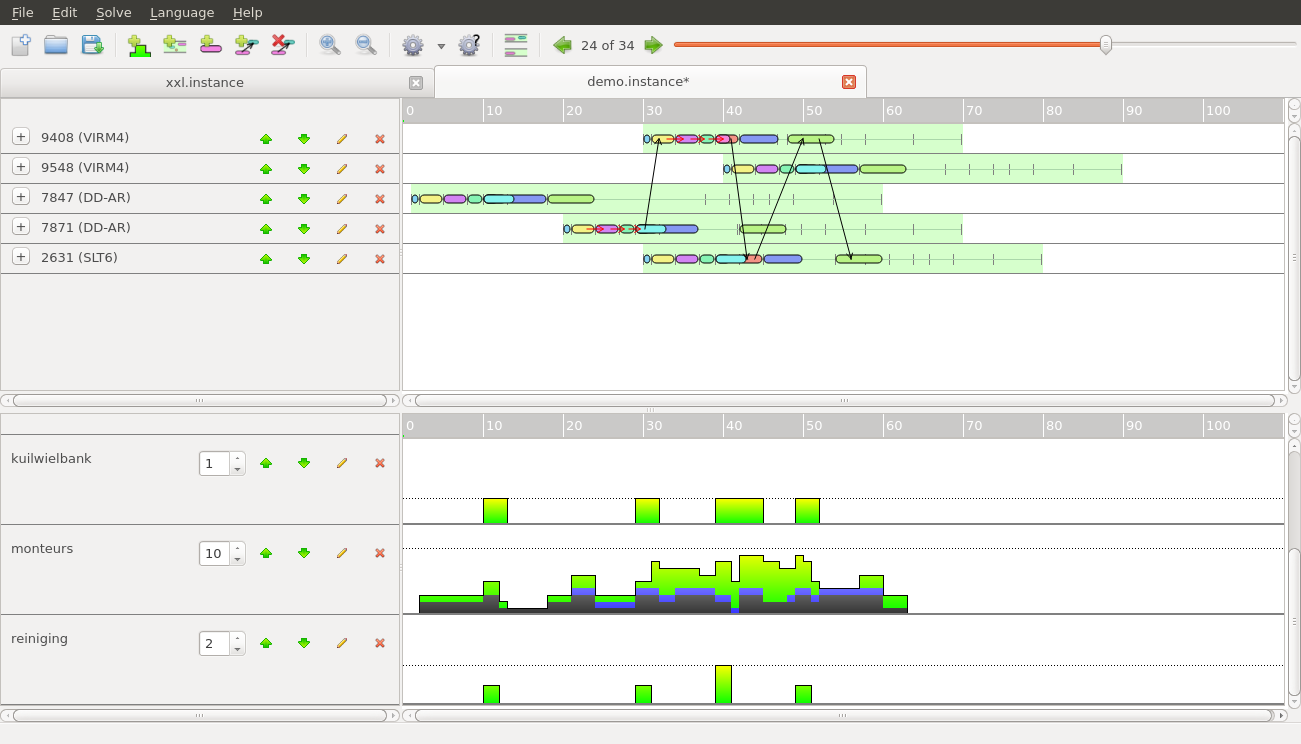
\includegraphics[width=.95\textwidth]{../images/GUIfinal.png}
\caption{De grafische gebruikersinterface.}
\label{fig:GUIfinal}
\end{figure}

In Figuur \ref{fig:GUIfinal} is in de rechterbovenhoek een schuifbalk te zien, waarmee verschillende stappen van het proces van de solver laten zien kunnen worden in de interface. Naar zo'n stap, waarin de toestand van alle activiteiten opgeslagen in, zal vanaf nu gerefereerd worden als een frame. De volgende frames worden toegevoegd na het uitvoeren van een solver:
\begin{itemize}
\item Een frame met de begintoestand van de instantie.
\item Voor elke voorrangsrelatie die tijdens het ESTA$^+$ algoritme toegevoegd wordt, een nieuw frame met daarop alleen de nieuwe voorrangsrelatie en eventuele veranderingen in starttijden van de activiteiten.
\item Een frame zonder voorrangsrelaties, waarin geen resource conflicten meer aanwezig zijn. Op dit moment worden alle eerder toegevoegde voorrangsrelaties verwijderd.
\item Voor elke resource een frame waarop alle bij deze resource horende chains getoond worden. Vervolgens een apart frame voor elke chain, die elk bij 1 resource unit hoort. Voor lege chains zal geen frame toegevoegd worden, maar voor chains met maar 1 activiteit wel.
\item Tenslotte een frame waarin voor elke activiteit in het blauw een flexibiliteitsinterval te zien is. Activiteiten worden ook verplaatst, zodat ze zich volledig in het blauwe interval bevinden.
\end{itemize}
Als een solver geen chains en/of flexibiliteitsintervallen berekent, zullen voor deze stappen geen frames worden toegevoegd en zullen alleen de frames van het ESTA$^+$-algoritme getoond worden.

In het frame dat in Figuur \ref{fig:GUIfinal} zichtbaar is, wordt een chain van activiteiten, behorende bij de resource 'monteurs', in het bovenste deelvenster getoond. Hierin zijn de rode pijlen voorrangsrelaties die al in de instantie aanwezig waren en zijn de zwarte pijlen later toegevoegd tijdens het oplossen van de instantie.

Zoals eerder genoemd, worden van een resource eerst alle chains tegelijk getoond op een frame, en vervolgens elke chain op een apart frame. Tijdens het \'e\'en voor \'e\'en laten zien van de chains, wordt  het profiel van de gebruikte resources stap voor stap opgebouwd. Op het moment dat er nog geen resources gebruikt worden, is het gehele profiel groen. Bij het tonen van een chain worden alle resource units die door de activiteiten in deze chain gebruikt worden, in het blauw getoond. Dit betekent dus dat deze resource units niet meer door andere activiteiten gebruikt kunnen worden. Deze gebruikte resources zijn dus in daarop volgende frames grijs gekleurd. Zo wordt in elke frame het grijs gekleurde gebied groter, totdat elke resource unit gebruikt is.

\subsubsection*{Flexibiliteitsintervallen}
Zoals in Figuur \ref{fig:flex-interval} is te zien, is het ook mogelijk om het flexibiliteitsinterval van elke activiteit weer te geven in de interface. Activiteiten kunnen vrij bewegen binnen het flexibiliteitsinterval zonder dat er conflicten ontstaan met andere activiteiten. Als de intervallen worden weergegeven, is het niet mogelijk om de activiteiten buiten het bijbehoorende interval te verplaatsen. Ook is het niet mogelijk activiteiten zodanig langer te maken dat ze buiten hun flexibiliteitsinterval vallen. Die twee ==dingen== zijn niet mogelijk om ervoor te zorgen dat het schema flexibel blijft. Als het weergeven van de flexibiliteitsintervallen wordt uitgezet kunnen de activiteiten wel verplaatst en vergroot worden buiten het flexibiliteitsinterval.

\begin{figure}[H]
\center
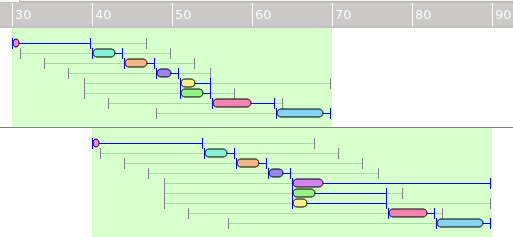
\includegraphics[width=.7\textwidth]{../images/flex-interval.png}
\caption{Flexibiliteitsintervallen}
\label{fig:flex-interval}
\end{figure}

\subsubsection*{Gebruiksgemak}
Om het gebruiksgemak te vegroten zijn er een aantal sneltoetsen toegevoegd. Ook is het sluiten van instanties veranderd, want waar eerst instanties gesloten konden worden met een grote rode knop in de menubalk, is er nu op elke tab van een instantie een klein kruisje geplaatst, waarmee de instantie gesloten kan worden. Dit ontwerp ziet er intu\"itief uit en wordt ook gebruikt door veel bekende browsers zoals Google Chrome en Mozilla FireFox.

Er zijn ook sneltoetsen toegevoegd voor het in- en uitzoomen en voor het horizontaal scrollen. Er kan in- en uitgezoomd worden door de ctrl-toets ingedrukt te houden en het scrollwiel van de muis  te bewegen. Horizontaal scrollen kan in het venster waarin de muis zich op dat moment bevindt door de shift-toets ingedrukt te houden en het scrollwiel van de muis te bewegen. Deze sneltoetsen zijn ingesteld zodat de gebruiker makkelijker door een probleeminstantie kan navigeren, zonder daarvoor steeds zijn muis naar de menubalk te hoeven verplaatsen.

Nog een feature die voor een verbeterd gebruiksgemak moet zorgen zijn de knopjes voor het van plek verwisselen van taken en resources. Dit is vooral handig als er een nieuwe activiteit of resource wordt toegevoegd, want deze worden altijd onderaan gezet. 

\subsection{Port naar Windows 7}
Om de toegankelijkheid van de applicatie te vergroten, is ervoor gezorgd dat deze ook op het besturingssysteem Windows 7 werkt. Hierbij is het ook nog steeds mogelijk om deze op Unix-based systemen te draaien, zoals Ubuntu. Alle functies van het programma moeten dus zowel op Windows 7 als op Ubuntu correct werken.

\subsection{Upgrade naar Qt 5.2}
De bestaande applicatie was ontwikkeld in versie 4.8 van het Qt framework, maar om de applicatie zo up-to-date mogelijk te houden, is deze geport naar Qt versie 5.2. Hierdoor hoeft een eventuele groep, die de applicatie verder gaat ontwikkelen, niet met een oude versie van het Qt framework te werken. Deze upgrade betekent echter ook dat de applicatie niet meer werkt met Qt 4, maar alleen met versie 5.

\newpage
\section{Performance}
Om de gebruikte oplossingsmethoden te verantwoorden, zullen deze in dit hoofdstuk vergeleken worden met andere mogelijke methoden. Zowel de looptijd van het oplossen van verschillende probleeminstanties zal geanalyseerd worden als de flexibiliteit die met verschillende methodes bereikt wordt.

\subsection{Looptijd}
TODO: Looptijd van interior point en update bestaande tabellen want blijkbaar stond debug aan.

In dit hoofdstuk een analyse van de looptijd van de solver. Bij deze analyse delen we de solver op in vijf belangrijke delen: parsen, STJN, ESTA$^+$, chaining en LP. Om de looptijd te bepalen gebruiken we een grote probleeminstantie genaamd 'xxl-instance'. Deze probleeminstantie bestaat uit:
\begin{itemize}
    \item 10 resources, met elk 1 resource unit
    \item 180 projecten, met elk tussen de 4 en de 6 activiteiten
    \item 912 activiteiten, die elk gebruik maken van tussen de 1 en 5 resources
\end{itemize}

In de Tabellen \ref{tbl:xxl+output}, \ref{tbl:xxl-output} en \ref{tbl:xxl+outputbestand} is te zien wat de looptijden zijn van de onderdelen van de solver met en zonder printen van output. Deze waarden komen van een getrimd gemiddelde van 20 metingen. De solver stuurt de output naar \texttt{stdout} Als er wel output wordt geprint duurt het oplossen van de 'xxl-instance' iets minder dan $110$ seconden en als er geen output wordt geprint duurt het oplossen ongeveer $1,4$ seconden. Ook valt op dat als alle output niet naar \texttt{stdout}, maar naar een bestand wordt gestuurd de totale looptijd iets minder dan $4$ seconden duurt. Er valt dus veel snelheidswinst te behalen door het printen te optimaliseren. Een andere optie is om slimmer om te gaan met wat er wel en niet wordt geprint, want dat kan ook al veel tijd schelen. Een mogelijkheid is om niet telkens alle informatie van een nieuw frame te printen, maar alleen het verschil met het vorige frame. Een andere mogelijkheid is om niet met een apparte solver te werken die wordt aangeroepen door de NedTrain Planner, maar de solver te integreren in de NedTrain Planner. Dan hoeft er niets te worden uitgeprint, maar dit heeft wel als nadeel dat er dan niet gemakkelijk een nieuwe solver toegevoegd kan worden aan de NedTrain Planner. Daarom is printen naar een tijdelijk bestand in plaats van \texttt{stdout} mogelijk een goed alternatief om voor een versnelling te kunnen zorgen. 

\begin{table}[H]
\parbox{.45\linewidth}{
    \centering
    \begin{tabular}{| l | r | r |}
        \hline
                    & Looptijd ($s$)  & Percentage ($\%$) \\
        \hline
        Parsing     & $0.010927$      & $0.0$   \\
        STJN        & $0.002788$      & $0.0$   \\
        ESTA$^+$    & $108.299420$    & $99.2$  \\
        Chaining    & $0.565354$      & $0.5$   \\
        LP          & $0.319607$      & $0.3$   \\
        \hline \hline
        Totaal      & $109.198681$    & $100.0$ \\
        \hline
    \end{tabular}
    \caption{xxl-instance met output}
    \label{tbl:xxl+output}
}
\hfill
\parbox{.45\linewidth}{
    \centering
    \begin{tabular}{| l | r | r |}
        \hline
                    & Looptijd ($s$)& Percentage ($\%$) \\
        \hline
        Parsing     & $0.010247$      & $0.7$   \\
        STJN        & $0.002798$      & $0.2$   \\
        ESTA$^+$    & $1.092032$      & $76.5$  \\
        Chaining    & $0.037414$      & $2.6$   \\
        LP          & $0.283970$      & $19.9$  \\
        \hline \hline
        Totaal      & $1.426638$      & $100.0$ \\
        \hline
    \end{tabular}
    \caption{xxl-instance zonder output}
    \label{tbl:xxl-output}
}
\end{table}

\begin{table}[H]
    \centering
    \begin{tabular}{| l | r | r|}
        \hline
                    & Looptijd ($s$)& Percentage ($\%$) \\
        \hline
        
        Parsing     & $0.009044$    & $0.2$     \\
        STJN        & $0.002736$    & $0.1$     \\
        ESTA$^+$    & $3.362071$    & $88.0$    \\
        Chaining    & $0.159881$    & $4.2$     \\
        LP          & $0.288064$    & $7.5$     \\
        \hline \hline
        Totaal      & $3.822129$    & $100.0$   \\
        \hline
    \end{tabular}
    \caption{xxl-instance en output naar bestand}
    \label{tbl:xxl+outputbestand}
\end{table}

\subsection{Flexibiliteit}
De verdeling van de flexibiliteit over alle activiteiten kan gemeten worden met de \emph{Mean Squared Error} (MSE) van de flexibiliteit $MSE(flex)$ die staat gedefinieerd in Formule \ref{eq:mse}. Hoe lager deze MSE is hoe beter de flexibiliteit is verdeeld over de activiteiten.

\begin{align}
\label{eq:mse}
\begin{aligned}
    flex_{gem} =& \sum_{t \in T} \frac{t^+ - t^-}{|T|}      & \text{met } |T| \text{ het aantal elementen in } T\\
    MSE(flex) =& \sum_{t \in T} (flex_t - flex_{gem})^2     & \\
               =& \sum_{t \in T} (t^+ - t^- - flex_{gem})^2 & \\
\end{aligned}
\end{align}

Er is met $2040$ probleeminstanties getest welke van de vier methodes de beste verdeling van flexibiliteit geeft. In Tabel \ref{tbl:performanceflex} worden telkens twee methoden vergeleken. 

\begin{table}[H]
    \centering
    \begin{tabular}{ r || r r r r }
            & \rot{interior 1} & \rot{interior 2} & \rot{simplex 1} & \rot{simplex 2} \\
        \hhline{=||====}
        interior 1 & $-$ & $0,0$ & $88,5$ & $-$ \\
        interior 2 & $99,9$ & $-$ & $-$ & $88,9$ \\ 
        simplex 1  & $10,5$ & $-$ & $-$ & $0,1$ \\
        simplex 2  & $-$ & $10,7$ & $99,9$ & $-$ \\
    \end{tabular}
    \caption{Vergelijking van de 4 verschillende methoden}
    \label{tbl:performanceflex}
\end{table}

Dus:
\begin{enumerate}
    \item interior 2
    \item interior 1
    \item simplex 2
    \item simplex 1
\end{enumerate}

\subsection{Chaining}
TODO: Hier komt nog een analyse van de verschillende methodes van chaining om een chain te selecteren. 

\newpage
\section{Ontwikkelproces}
\subsection{Ontwikkelmethode}
Tijdens de ontwikkeling van de NedTrain Planner en de solvers is er zoveel mogelijk gebruik gemaakt van de scrum principes. Meestal waren features aan het eind van een sprint geschikt voor een mogelijke demo, maar zaten er nog wel een aantal bugs in. Het meest voorkomende probleem was dat een feature aan het einde van de sprint nog niet werkte op een Windows computer.

\subsubsection{Sprint 1}
Het doel van de eerste sprint was om het chaining algoritme te implementeren. Tijdens de onderzoeksfase hebben we gezien dat het beschikbaar maken voor Windows 7 waarschijnlijk goed te doen is in de tijd die daarvoor beschikbaar was. Het porten van de NedTrain Planner naar Windows 7 was daarom ook een doel in de eerste sprint. 

\textbf{Terugblik} \\
We zijn er tevreden over het verloop van de eerste sprint. Het porten naar Windows 7 liep met een paar kleine tegenvallers redelijk vlot. Naast het porten naar Windows 7 is het ook in deze sprint gelukt om de versie van Qt te upgraden naar versie 5.2.1. De basis van ons chaining algoritme werkt, maar de samenwerking tussen GUI en Solver loopt nog niet zoals gewenst. Er is zelf ook al een begin gemaakt aan de LP Solver, een doel dat voor de tweede sprint gepland stond. 

\subsubsection{Sprint 2}
Het voornaamste doel van de tweede sprint is de COIN-OR LP solver te laten samenwerken met onze applicatie. Daarnaast is er gewerkt aan het laten zien van aparte chains met daarbij welke resources er door deze chain gebruikt worden. 

\textbf{Terugblik} \\
In deze sprint hebben we een aantal tegenvallers gehad. Zo hadden we last van een memory leak, wat redelijk veel tijd kostte om op te lossen. Bovendien moest de bestaande architectuur voor het laten zien van chains vrij veel aangepast worden. Een tweede tegenvaller was het updaten van de software op de Jenkins-server. Aangezien we de tools hebben ge\"upgrade naar Qt versie 5.x, moet op de server Qt ook worden ge\"upgraded. Dit ging niet meteen de eerste keer goed, waarbij uiteindelijk is overgegaan tot een volledige herinstallatie. Dit heeft als gevolg dat we een deel van de eerste commits missen in de continuous integration grafiek.

\subsubsection{Sprint 3}
In deze sprint zullen we een demo geven aan onze opdrachtgevers. Hiermee kunnen we controleren of wat wij hebben gemaakt de opdrachtgevers ook echt willen. We kunnen dan nog het \'e\'en en ander aanpassen in deze en volgende sprints.

\textbf{Terugblik} \\
Het is in deze sprint gelukt om per chain te laten zien welke resources er door de activities in deze chain gebruikt worden. Elke chain kan apart op een frame getoond worden, waarbij de resource units die door deze chain gebruikt zijn, blauw gekleurd worden. De resource units die door eerdere chains van deze resource gebruikt zijn, zijn zwart gekleurd. Dit hebben we tijdens de demo laten zien. De feedback die hierover gegeven was, was dat er niet heel makkelijk gezien kan worden welke taken bij een bepaalde resource unit, bijvoorbeeld een monteur, horen. Om dit duidelijker te maken, zou een aparte view gemaakt kunnen worden. Hierin is echter minder makkelijk te zien hoeveel resources er op een bepaald tijdstip gebruikt worden.

De CLP solver is in deze sprint ook veel verder gevorderd. Er bestaat niet meer een aparte binary voor de CLP solver, maar deze is ge\"integreerd in de binary van de chaining solver. Er kan een willekeurige LP instantie als input gegeven worden en deze kan door de solver opgelost worden. Wat nu nog overblijft is het transformeren van een RCPSP instantie naar een LP instantie, zodat deze opgelost kan worden.

\subsubsection{Sprint 4}
In deze sprint hebben we als doel om de flexibiliteitsintervallen, die worden berekend m.b.v. de LP-solver, door te geven aan de gebruikersinterface. Ook is het belangrijk om dit op een goede manier weer te geven, zodat de gebruiker deze informatie op een juiste manier kan interpreteren. Tenslotte willen we de tool zo compileren, dat de gebruiker het gemakkelijk kan installeren. Hiervoor moet de tool statisch gelinkt worden met de gebruikte libraries. Op deze manier kan de applicatie uitgevoerd worden, zonder dat er nog andere software ge\"installeerd moet worden.

\textbf{Terugblik} \\
Het is ons gelukt om in deze sprint de flexibiliteitsintervallen weer tegeven op het scherm, maar de gebruiker kan dit nog niet aan- en uitzetten. Het verder doorontwikkelen van de features rondom de flexibiliteitsintervallen krijgt een hoge prioriteit in de volgende sprint. De NedTrain Planner kan nu zeer gemakkelijk ge\"installeerd worden op Windows 7, maar voor computers met Linux werkt dit helaas nog niet. 

\subsubsection{Sprint 5}
In deze sprint is het belangrijk de feature van het weergeven van de flexibiliteit af te maken en te testen. Aan het einde van deze sprint moet de code worden opgestuurd naar SIG en moet er een eerste versie van het eindverslag af zijn. 

\textbf{Terugblik} \\
We hebben deze sprint veel tijd moeten besteden aan het verslag, maar we hebben gelukkig ook tijd kunnen besteden aan het verder door ontwikkelen van de NedTrain Planner. In deze sprint hebben we de code kwaliteit verbeterd en bugs ontdekt de vorige groep heeft achter gelaten. Deze bugs hebben we ook meteen weten te verhelpen.

\subsubsection{Sprint 6}
Aan het begin van deze sprint gaan we weer een demo doen, zodat de klant kan zien waar het product nu staat. Bij grote instanties loopt de interface vast bij het tekenen van de flexibiliteitsintervallen, we moeten proberen dit effeci\"enter te doen.

\textbf{Terugblik} \\
Na de demo hebben wij besloten om nog \'e\'en laatste feature te implementeren, omdat dit voor de opdrachtgever een vrij hoge prioriteit had. Dit is de rooster feature, die de werking van het chaining algoritme duidelijk maaakt. De interface loopt niet meer vast als er bij grote instanties flexibiliteitsintervallen getekend moeten worden. Verder hebben we een aantal bugs verholpen en het verslag afgemaakt. 

\subsection{Hulpmiddelen}
Zoals beschreven in het Plan van Aanpak en het Ori\"entatieverslag hebben we voor een aantal hulpmiddelen gekozen of moeten gebruiken. In deze sectie wordt onze ervaring van het gebruik van deze hulpmiddelen besproken, maar ook een aantal resultaten daarvan. 

\subsubsection{Versiebeheer}
\label{subsec:versiebeheer}
Als versiebeheersysteem is voor dit project een Git repository gebruikt op de website \href{http://bitbucket.com}{Bitbucket.com}. Hiervoor hadden wij gekozen, omdat wij het meest bekend zijn met Git. Toch hebben wij nog veel bijgeleerd en gaat het gebruik ons steeds makkelijker af. Het is ons gelukt om altijd een werkende master branch te hebben. Dit heeft als grote voordeel dat er op elk moment tijdens het ontwikkelproces een demo gehouden kan worden. Ook is dit belangrijk om de tests op de continuous intregration server te laten slagen. Doordat de tool moet blijven werken op zowel Windows 7 als Linux, werden nieuwe features relatief laat aan de master branch toegevoegd. Vaak ontwikkelden we een nieuwe feature op een computer met Ubuntu en gingen pas als het af is de problemen op Windows 7 verhelpen.

\subsubsection{Continuous Integration}
Wij hebben continuous integration willen toepassen door gebruik te maken van een Jenkins server. Deze server werd door onszelf beheerd en stond fysiek bij \'e\'en van de projectleden thuis. Het heeft erg veel tijd gekost om alle software, die nodig is voor het compileren van dit project, te installeren. Zoals vermeld staat in sectie '\nameref{subsec:versiebeheer}', hebben we relatief laat nieuwe features toegevoegd aan de master branch. Dit heeft als gevolg dat de master branch weinig verandert en het daardoor weinig zin heeft om elke dag te builden. Ook zijn er problemen ontstaan bij het upgraden naar Qt versie 5. Het upgraden van de software op de server ging gepaard met veel problemen en er is uiteindelijk overgegaan tot herinstallatie van de server. In sprint 5 zijn er wederom problemen ontstaan toen de server een keer opnieuw werd opgestart, hierdoor zijn wij de build geschiedenis kwijtgeraakt. Al met al heeft het toepassen van continuous integration veel tijd gekost en weinig opgeleverd. 

\subsubsection{Google Test}
Het project had, voordat wij dit hebben uitgebreid, al een flinke hoeveelheid tests, maar er waren nog veel klassen waar helemaal geen tests voor zijn gemaakt. Wij hebben voor zowel nieuwe features, als bestaande features zonder tests, tests gemaakt. De solver had helemaal geen tests. Een uitgebreide testsuite is ook belangrijk voor de klant, zo kunnen volgende ontwikkelaars gemakkelijk op dit project voortbouwen zonder ongemerkt onderdelen kapot te maken. 

Alle tests die zijn gemaakt maken gebruiken van het Google Test framework. Dit was erg prettig in gebruik en het uitbreiden van de testsuite ging redelijk eenvoudig. We hebben er voor gekozen om voor de solver een apparte testsuite te maken en deze niet te integreren met de bestaande testsuite voor de interface. Dit heeft als voordeel dat de testsuites net als de interface en solver zelf appart gebruikt kunnen worden. Voor de solver hebben we $42$ tests gemaakt. 

Om te zien of onze testsuite uitgebreid genoeg is hebben we de \emph{Code Coverage Tool} \texttt{gcovr} gebruikt. Deze tool geeft per bestand aan hoeveel regels code en branches er zijn uitgevoerd door de testsuite. Deze tool heeft ons gestimuleerd om meer testcases te schrijven, om daarmee een hogere dekking te bereiken. De resultaten van de analyse van deze tool zijn te vinden in Tabel \ref{tbl:covr-solver}. Het percentage branches dat wordt getest door de testsuite met een gemiddelde van $56,1\%$ te laag. Het percentage van regels code dat wordt getest door de testsuite is met een gemiddelde van $76,\%$ wel redelijk.

\begin{table}[H]
    \centering
    \begin{tabular}{| l | r | r |}
        \hline
        Bestand & \midden{Regels $(\%)$} & \midden{Branches $(\%)$} \\
        \hline
        \texttt{chaining.cpp}    & $87,2$   & $58,1$ \\ 
        \texttt{constraints.cpp} & $100,0$  & $56,6$ \\
        \texttt{esta\_plus.cpp}  & $69,3$   & $56,0$ \\
        \texttt{exceptions.cpp}  & $62,5$   & $50,0$ \\
        \texttt{flexibility.cpp} & $99,0$   & $53,2$ \\
        \texttt{heap.cpp}        & $54,7$   & $58,3$ \\
        \texttt{output.cpp}      & $68,8$   & $50,0$ \\
        \texttt{solve.cpp}       & $65,2$   & $50,0$ \\
        \texttt{stjn.cpp}        & $68,9$   & $57,8$ \\
        \texttt{timing.cpp}      & $79,6$   & $63,6$ \\
        \texttt{tmsp.cpp}        & $95,5$   & $55,9$ \\
        \hline
        \hline
        Gemiddelde               & $76,8$   & $56,1$ \\
        \hline
    \end{tabular}
    \caption{Code coverage van Solver}
    \label{tbl:covr-solver}
\end{table}

\subsubsection{\cpp\ en Qt}
Met \cpp\ hadden wij geen of nauwelijks geen ervaring, dus door deze programmeertaal te gebruiken hebben wij tijdens dit project veel kunnen leren. Het debuggen van \cpp -code vinden wij wel lastiger dan bijvoorbeeld bij een programmeertaal als JAVA. Vooral als het gaat om de \emph{Segmentation fault}, waarbij er weinig informatie wordt gegeven over wat er nou precies fout gaat. Toch zouden wij \cpp\ wel willen gebruiken bij volgende projecten, vooral als een goede performance een eis van de opdrachtgever is. 

Van Qt hadden wij nog nooit van gehoord, maar dit zouden we zeker vaker willen gaan gebruiken. We vinden Qt prettig werken en levert grafisch mooie gebruikersinterfaces op. Het was prettig om te beginnen met een bestaande applicatie, omdat dan sneller duidelijk is hoe bepaalde functies werken in Qt. Het was echter niet altijd prettig om aan een bestaande applicatie te werken, omdat het ontdekken en verhelpen van bugs in een groot project moeilijker is. 

\subsection{Software Improvement Group}
Aan het eind van sprint 5 is al onze code opgestuurd naar de Software Improvement Group, die op de code feedback en een beoordeling van 1 tot 5 sterren zal geven. De code wordt op de volgende onderdelen beoordeeld \cite{sigmanual}:
\begin{itemize}
\item \textbf{Volume} - Hoe meer regels code een applicatie bevat, hoe moeilijker het wordt om deze te onderhouden.
\item \textbf{Duplication} - Het kopi\"eren van code moet zo veel mogelijk vermeden worden.
\item \textbf{Unit size} - Het grootste deel van de applicatie moet bestaan uit units van maximaal 20 regels.
\item \textbf{Unit complexity} - De cyclomatische complexiteit, gemeten d.m.v. het \emph{McCabe complexity number}, moet voor het grootste deel van de code niet hoger zijn dan 5.
\item \textbf{Unit interfacing} - Het meegeven van meer dan 2 parameters moet zo veel mogelijk vermeden worden.
\item \textbf{Module coupling} - Het sterk gekoppeld zijn van verschillende groepen units moet vermeden worden, omdat dit de software moeilijker te onderhouden maakt.
\item \textbf{Component balance} - Alle componenten moeten ongeveer even groot zijn. Dit onderdeel wordt beoordeeld d.m.v. de \emph{adjusted Gini coefficient}.
\item \textbf{Component independence} - Er moet gestreefd worden naar zo veel mogelijk componenten die niet aangeroepen worden door componenten van andere modules. Alleen interface klassen zouden de communicatie tussen verschillende modules moeten regelen.
\end{itemize}

Van de code die op vrijdag 13 juni is opgestuurd, is het volgende commentaar op ontvangen.

\begin{tabular}{p{0.5cm} | p{\textwidth - 2cm} |}
\cline{2-2}
 & \\ & \setlength{\parskip}{5pt}
De code van het systeem scoort bijna 4 sterren op ons onderhoudbaarheidsmodel, wat betekent dat de code bovengemiddeld onderhoudbaar is. De hoogste score is niet behaald door een lagere score voor Module Coupling, Unit Size en Unit Complexity.

Voor Module Coupling wordt er gekeken naar het percentage van de code wat relatief vaak wordt aangeroepen. Normaal gesproken zorgt code die vaak aangeroepen wordt voor een minder stabiel systeem omdat veranderingen binnen dit type code kan leiden tot aanpassingen op veel verschillende plaatsen. In dit systeem wordt bijvoorbeeld de relatief grote file 'instance\_misc' op ruim $160$ verschillende plaatsen gebruikt. Een ander voorbeeld is 'instance\_manip.cpp', $1$ van de grootste files in het systeem welke op ruim $60$ plaatsen gebruikt wordt. Het lijkt erop dat deze files verschillende functionaliteiten bevatten, daarnaast is het uit de naamgeving niet duidelijk welke functionaliteit waar geïmplementeerd zou moeten zijn. Om zowel de grootte als het aantal aanroepen te verminderen zouden deze functionaliteiten gescheiden kunnen worden, wat er ook toe zou leiden dat de afzonderlijke functionaliteiten makkelijker te begrijpen, te testen en daardoor eenvoudiger te onderhouden worden.

Voor Unit Size wordt er gekeken naar het percentage code dat bovengemiddeld lang is. Het opsplitsen van dit soort methodes in kleinere stukken zorgt ervoor dat elk onderdeel makkelijker te begrijpen, te testen en daardoor eenvoudiger te onderhouden wordt. Binnen de langere methodes in dit systeem, zoals bijvoorbeeld de 'esta\_plus'-methode, zijn aparte stukken functionaliteit te vinden welke ge-refactored kunnen worden naar aparte methodes. De body van condities of de 'cleanup' code zijn hier voorbeelden van. Het is aan te raden kritisch te kijken naar de langere methodes binnen dit systeem en deze waar mogelijk op te splitsen.

Voor Unit Complexity wordt er gekeken naar het percentage code dat bovengemiddeld complex is. Ook hier geldt dat het opsplitsen van dit soort methodes in kleinere stukken ervoor zorgt dat elk onderdeel makkelijker te begrijpen, makkelijker te testen en daardoor eenvoudiger te onderhouden wordt. In dit geval komen de meest complexe methoden ook naar voren als de langste methoden, waardoor het oplossen van het eerste probleem ook dit probleem zal verhelpen.

Over het algemeen scoort de code bovengemiddeld, hopelijk lukt het om dit niveau te behouden tijdens de rest van de ontwikkelfase. De aanwezigheid van test-code is in ieder geval veelbelovend, hopelijk zal het volume van de test-code ook groeien op het moment dat er nieuwe functionaliteit toegevoegd wordt. 

\hfill Software Improvement Group \\
\cline{2-2}
\end{tabular}

\newpage
\section{Discussie en Aanbevelingen}
De vorige bacheloreindprojectgroep beveelde een undo-functionaliteit aan voor de applicatie \cite{bep2012nedtrain}. Wij zien ook zeker het voordeel van een undo-functionaliteit in, omdat bij het gebruik wel eens iets per ongeluk verwijderd of veranderd wordt. Aangezien de NedTrain Planner nu meer wordt gebruikt voor onderzoek en educatie, wordt de focus toch gelegd op andere belangrijke features. Als deze tool gebruikt gaat worden door NedTrain, is een undo-functionaliteit een must-have. We hebben onderzocht hoe deze feature gemaakt zou kunnen worden. Een voordeel is dat Qt een Undo Framework heeft, maar om dit te kunnen gebruiken moet er veel aan de code veranderd worden. 

Vervolgens raden we ook het verbeteren van de kwaliteit van de code aan. Bij het implementeren van nieuwe functionaliteiten hebben we namelijk soms gemerkt dat de huidige structuur van de applicatie niet ideaal was. Voor de bestaande functionaliteiten was de structuur wel geschikt, maar dus niet altijd voor de nieuwe features. Voor het toevoegen van sommige nieuwe functionaliteiten zou het beter zijn om de structuur van het gehele programma te veranderen, maar vanwege beperkte tijd is dit niet uitgevoerd.

Als derde aanbeveling zou het goed zijn om de communicatie tussen de solver en de interface te verbeteren. De grootste snelheidswinst is nu te behalen in de communicatie tussen de NedTrain Planner en de solver. Er kan worden gekeken naar de uitvoer van de solver tijdelijk naar een bestand te schrijven en deze daarna in te lezen door de NedTrain Planner. Ook kan de hoeveelheid informatie die wordt verstuurd van de solver naar de NedTrain Planner worden gereduceerd. Van elk frame dat wordt getoond door de interface, worden alle starttijden van de activiteiten door de solver uitgeprint, ook al verandert er maar \'e\'en activiteit. Door steeds het verschil tussen het huidige en het vorige frame door te geven, valt een relatief grote snelheidswinst te behalen.

Een vierde aanbeveling is een feature toe te voegen waarbij de resources zo eerlijk mogelijk verdeeld worden over de resource units. Dit is vooral handig voor personeel in de werkplaatsen van NedTrain. Zo kan elk personeelslid voor elk moment van de dag zien aan welk project hij of zij werkt en wanneer zijn of haar pauzes zijn. Belangrijk is ook om er rekeningen mee te houden dat deze resources mensen zijn. Ze kunnen niet te lang achter elkaar werken en hebben na een bepaalde tijd pauze nodig. Elke rij hoort bij een werknemer/resource unit en elke kolom bij een tijdseenheid. Een groen ingekleurd vlak betekent dat de werknemer aan het werk is. In Figuur \ref{fig:schema} wordt getoond dat de taken nu slecht verdeeld worden over de resource units. In het voorbeeld in Figuur \ref{fig:schema} worden aan \'e\'en resource unit helemaal geen taken toegekend. 

\begin{figure}[H]
\centering
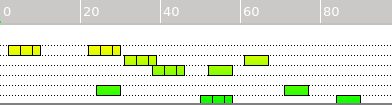
\includegraphics[width=.5\textwidth]{../images/schedule.png}
\caption{Resource unit schema}
\label{fig:schema}
\end{figure}

\newpage
\section{Conclusie}
Achteraf gezien kunnen we een aantal conclusies trekken over dit project. In het Plan van Aanpak wordt een aantal op te leveren features genoemd, onderverdeeld in drie categori\"en van prioriteit. Alle taken met hoge prioriteit zijn volbracht en in de categorie met taken van gemiddelde prioriteit stond de undo-functionaliteit, die wij niet hebben kunnen implementeren door een gebrek aan tijd. We hebben onderzocht wat er nodig zou om deze functionaliteit te \"implementeren en kwamen tot de conlusie dat dit erg veel tijd zou gaan kosten en niet in verhouding zou staan met wat het zou opleveren. In de categorie lage prioriteit hebben we alles kunnen doen, behalve \emph{"Het verduidelijken van het vergelijken van verschillende oplossingen."} We zijn erg tevreden nu we kunnen concluderen dat we zoveel features hebben kunnen maken.

We hebben allen veel geleerd van de programmeertaal \cpp\ en het Qt framework. Deze waren beide voor ons erg onbekend en vooral \cpp\ leverde soms aardig wat hobbels op in de weg naar succes. 

De samenwerking liep gesmeerd, dit mede doordat wij ook al aan een eerder project hebben samengewerkt. De feedback van onze begeleiders heeft ook zeker bijgedragen aan een beter eindproduct. Het feit dat andere groepen al aan dit project hebben gewerkt en zeer waarschijnlijk ook wij opgevolgd zullen worden door enthousiaste informatici maakt dit project realistischer dan elk ander project tijdens de bacheloropleiding. Wij vonden dit allen een zeer leerzaam en geslaagd Bachelorproject.


\newpage
\addcontentsline{toc}{section}{Referenties}
\bibliographystyle{abbrv}
\bibliography{../references}

\fancyhead{}

\newpage
\begin{appendices}
\section{Opdrachtomschrijving} \label{app:A}
\subsection*{Project description}
NedTrain has developed a scheduling tool for operational maintenance. This tool consists of a scheduler and and extensive user interface. The proposed project consists in extending the current solver to construct flexible schedules for maintenance jobs. The proposed activities are.

\begin{enumerate}
	\item The addition of constraint posting techniques that provide a set of temporal constraints ensuring the satisfaction of all resource constraints.
	\item The use of an LP solver to measure the flexibility of the resulting constraint system.
	\item The extension of the user interface to provide the user with flexibility information and to evaluate the changes in flexibility after the users feedback.
\end{enumerate}

\subsection*{Company description}

NedTrain is a part of NS Group, which is the largest railway operator in the Netherlands. NS Group can be decomposed in three important parts: railway station exploitation, train maintenance and of course passenger transportation. NedTrain, which performs rolling stock maintenance, is currently contracted to perform maintenance for the rolling stock used by nsr and NS HiSpeed. The fleet used by these two divisions has a size of around 3000 passenger carriages, of which some 250 are under some form of maintenance at any one time. Maintenance operations are spread out over 37 locations throughout the Netherlands. The core task of NedTrain is guaranteeing fleet availability in the broadest sense of the word. Firstly, this means that trains should have as few breakdowns during service as possible. To ensure this, NedTrain has to focus on the quality of their maintenance work.

\subsection*{Auxiliary information}

This information has been provided by me (Cees Witteveen) after consulting Bob Huisman MSc, the director of research at NedTrain Company: bob.huisman@nedtrain.nl
\newpage

\section{Plan van Aanpak} \label{app:B}
\newpage

\includepdf[pages=-]{../plan_van_aanpak/verslag.pdf}

\section{Ori\"entatieverslag} \label{app:C}
\newpage

\includepdf[pages=-]{../orientatieverslag/verslag.pdf}

\section{Requirementsanalyse} \label{app:D}
\newpage

\includepdf[pages=-]{../requirementsanalyse/verslag.pdf}

\end{appendices}


\end{document}
